\setcounter{page}{1} % Iniciar la numeración de las páginas en este punto

\section{Introducción}


\section{Antecedentes}

    \subsubsection*{A chest-based continuous cuffless blood pressure method: Estimation and evaluation using multiple body sensors \cite{bodySensor}.}

    El artículo analiza el desarrollo de un dispositivo no invasivo para la estimación de la presión arterial (PA) utilizando sensores colocados en el pecho utilizando la bioimpedancia (BImp) como alternativa a la fotopletismografía (PPG) para la extracción del tiempo de llegada del pulso (PAT), se tomaron cinco lecturas de tiempo de pulso diferentes y se pudo estimar la PA sistólica y diastólica. 
    
    Se analizaron los datos de 41 participantes en diversas condiciones fisiológicas, incluidos los cambios de postura y los resultados mostraron que la combinación de PAT con la frecuencia cardíaca 
    mejoró la precisión del cálculo de la PA, y las lecturas de PAT basadas en BImp fueron un 3\% más precisas que las basadas en PPG, lo que destaca el potencial de BImp para un control más eficaz de la PA.

    \subsubsection*{An Arterial Compliance Sensor for Cuffless Blood Pressure Estimation Based on Piezoelectric and Optical Signals \cite{piezoelectric}.}

    Este artículo propone el desarrollo de un pequeño sistema de monitoreo que integra una matriz de sensores piezoeléctricos y un sensor óptico que monitorea las señales fisiológicas de la arteria radial. El sistema hace el cálculo del tiempo de tránsito del pulso (PTT) y correlaciona la ecuación de Moens-Korteweg con la velocidad de onda de pulso (PWV) para estimar la presión arterial sistólica (PAS) y diastólica (PAD).

    En un experimento con 20 participantes se compararon dos métodos de estimación de la presión arterial, el primero utilizando el modelo de regresión y el segundo modelo $P-\beta$ basado en la ecuación de Moens-Korteweg.

    \subsubsection*{Development of IoT Based Cuffless Blood Pressure Measurement System \cite{Norsuriati_2021}.}

    El artículo presenta el desarrollo de un sistema IoT de medición de presión arterial sin uso de un baumanómetro, se propone un método basado en el tiempo de tránsito del pulso (PTT). Este método correlaciona el tiempo de retraso entre las señales fotopletismografía (PPG) registrada en la punta del dedo y el lóbulo de la oreja.

    Los datos son recolectados mediante un microcontrolador Arduino Uno y procesados con el software MATLAB para eliminar el ruido y obtener los picos de la señal PPG para calcular el PTT.
    
    Los resultados son mostrados en la aplicación ThinkSpeak y ThingView debido a que tiene la capacidad de almacenar y visualizar los datos en tiempo real. El error medio y la deviación estándar para la presión arterial sistólica (PAS) estimada es de $22,5 \pm 20,6$ mmHg y para la presión arterial diastólica (PAD) es de $1,6 \pm 1,2$ mmHg.

    \subsubsection*{Diseño de un sistema internet de las cosas (IoT) para el monitoreo de la presión arterial \cite{Estrada_2021}. }

    En este artículo se presenta los procesos de diseño y construcción de un prototipo biomédico IoT para el monitoreo de la presión arterial de pacientes en su lugar de residencia. El sistema consta en colocar un brazalete en el paciente a la altura del corazón, al cual se conecta una bomba de aire que infla el brazalete, junto con un sensor de presión diferencial MPX5050DP. Los datos obtenidos son convertidos de analógico a digital mediante un microcontrolador y enviados, a través de una API REST, al servidor web IoT ThinkSpeak, donde se almacenan y pueden visualizarse en tiempo real.

    \subsubsection*{Development of Real-Time Cuffless Blood Pressure Measurement Systems with ECG Electrodes and a Microphone Using Pulse Transit Time (PTT) \cite{Electrodes_Microphone}.}

    El estudio habla sobre el desarrollo de un sistema de medición de la presión arterial en tiempo real sin uso de un baumanómetro, utilizando electrodos de ECG y un micrófono en lugar de un sensor de fotopletismografía (PPG). El sistema mide la onda de pulso sanguíneo en la arteria radial de la muñeca, calculando la presión arterial sistólica (SBP) y diastólica (DBP) mediante el tiempo de tránsito del pulso (PTT) entre el pico R del ECG y puntos característicos de la onda de pulso.
    
    Las estimaciones de SBP y DBP fueron comparables a las de un monitor de presión arterial comercial, con un error absoluto medio (MAE) de $2.72 \pm 3.42$ mmHg para SBP y $2.29 \pm 3.53$ mmHg para DBP.


\newpage
\section{Justificación}

En México, las enfermedades cardiovasculares representan la primera causa de muerte, siendo responsable de más de 220 mil fallecimientos en 2021 \cite{SSFallecimientos}. Entre los factores de riesgo más importantes para estas patologías se encuentra la hipertensión arterial, conocida también como el ``asesino silencioso", ya que no presenta síntomas y puede pasar desapercibida durante años, hasta que desarrollan complicaciones graves como infartos o accidentes cerebrovasculares. Según la Encuesta Nacional de Salud y Nutrición (ENSANUT), cerca del 30\% de la población adulta en México padece hipertensión arterial \cite{ENSANUT}, pero una gran proporción de ellos no recibe un tratamiento adecuado o no se diagnostica a tiempo debido a la falta de acceso a un monitoreo continuo y preciso.

Los métodos para la medición de la presión arterial, como el baumanómetro, son invasivos y requieren de personal capacitado, lo que limita su uso en el monitoreo continuo de la presión arterial. Esta limitación es crítica en un país como México, donde el sistema de salud puede ser limitado, especialmente en zonas rurales y marginadas. Por lo tanto, es necesario desarrollar dispositivos no invasivos y de bajo coste que permitan a las personas monitorear su presión arterial de forma continua y precisa, para detectar y tratar a tiempo la hipertensión arterial y de esta forma prevenir complicaciones graves.

Este proyecto tiene como objetivo desarrollar un sistema basado en sensores para la estimación de la presión arterial de forma no invasiva, que permita a las personas monitorear su presión arterial de forma continua y precisa, y enviar los datos a un dispositivo móvil para la visualización y el almacenamiento de los registros para llevar un control de su salud cardiovascular. Facilitando así la detección temprana de la hipertensión arterial y la prevención de complicaciones graves asociadas a esta enfermedad.

El desarrollo de un sistema de monitoreo no invasivo de la presión arterial permitirá a las personas tener un mayor control de su salud cardiovascular, detectar a tiempo la hipertensión arterial y prevenir complicaciones graves asociadas a esta enfermedad, mejorando así su calidad de vida y reduciendo la carga de enfermedades cardiovasculares en México.


\newpage
\section{Objetivos}
    \subsection{Objetivo General}
    Desarrollar un dispositivo para estimar la presión arterial de forma no invasiva utilizando sensores.
    \subsection{Objetivos Específicos}
    \begin{itemize}
        \item Diseñar un dispositivo utilizando sensores para la obtención de datos fisiológicos.
        \item Enviar los datos mediante Bluetooth a un dispositivo móvil.
        \item Procesar los datos obtenidos para la estimación de la presión arterial.
        \item Visualizar los datos obtenidos en una aplicación android.
    \end{itemize}

\newpage
\section{Marco Teórico}

    \subsection{El sistema de conducción del corazón}

    El corazón es un músculo que late y bombea continuamente sangre al resto del cuerpo. Lo que comúnmente llamamos latido cardíaco es en realidad la contracción rítmica de las cuatro cavidades del corazón. Cada latido cardíaco es estimulado por señales eléctricas que viajan a través de una vía específica del corazón. Estas señales se pueden registrar mediante un electrocardiograma (ECG).

     Este proceso comienza en el nódulo senoauricular (nódulo SA), situado en la aurícula derecha. La señal eléctrica se propaga a las aurículas, provocando su contracción y el empuje de sangre hacia los ventrículos. Luego, la señal llega al nódulo auriculoventricular (nódulo AV) y se desplaza a través del haz de His, que se divide en ramas izquierda y derecha dentro de los ventrículos. Finalmente, la señal viaja por las fibras de Purkinje, que son fibras musculares especializadas que se encuentran en las paredes de los ventrículos, el cual provoca la contracción de los ventrículos, bombeando sangre a los pulmones y al resto del cuerpo. Este sistema actúa como el marcapasos natural del cuerpo, manteniendo un ritmo cardíaco normal de 60 a 100 latidos por minuto. Alteraciones en este sistema pueden resultar en ritmos cardíacos anormales y afectar el flujo sanguíneo del cerebro y otras partes del cuerpo \cite{SistemaConduccionMSD}.

    \begin{figure}[H]
        \centering
        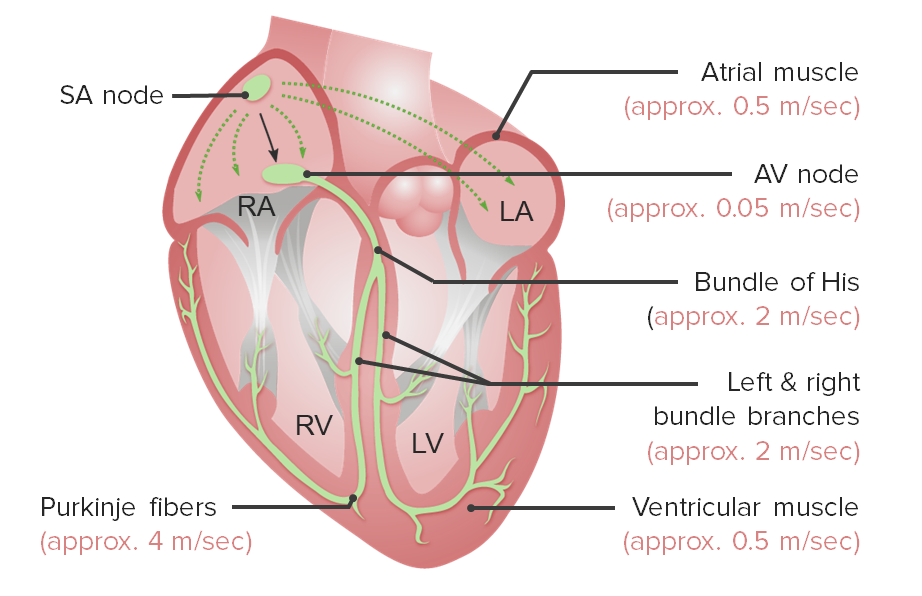
\includegraphics[width=0.7\textwidth]{img/sistemaConduccion.png}
        \caption[Sistema de conducción cardíaca y tiempos de conducción de los respectivos segmentos]{Sistema de conducción cardíaca y tiempos de conducción de los respectivos segmentos\footnotemark}
        \label{fig:sistemaConduccion}
    \end{figure}
    \footnotetext{Localización de las células marcapasos dentro del sistema de conducción del corazón. Imagen tomada de lecturio.com. [En línea]. Disponible en: \url{https://goo.su/MSZMxUj}}

    \subsection{Electrocardiograma (ECG)}
    Un electrocardiograma (ECG) es un estudio que registra el voltaje generado por los vectores de despolarización y repolarización de las células cardiacas en relación con el tiempo, es una herramienta útil para evaluar la función cardíaca y detectar problemas cardíacos \cite{ECG_Definicion}.

    Es una prueba no invasiva e indolora, que se realiza para detectar problemas cardíacos o controlar el estado del corazon. El ECG generalmente utiliza sensores (electrodos), colocados sobre la piel del pecho, pueden detectar señales eléctricas del corazón. Las señales de estos sensores se conectan a circuitos electrónicos simples con amplificadores, filtros y convertidores analógico-digitales, que registran la señal eléctrica y la muestran en un monitor o la imprimen para su posterior análisis.

    Las ondas del ECG son las siguientes:

    \begin{itemize}
        \item \textbf{Onda P}: Representa la despolarización auricular, es la suma de los vectores de despolarización de ambas aurículas.
        \item \textbf{Intervalo PR}: Representa el tiempo transcurrido desde la despolarización auricular, hasta la despolarización ventricular. Incluye la onda P y el segmento PR. Éste último elemento es una línea isoeléctrica, establecida gracias al retardo fisiológico que sufre la conducción eléctrica en el nodo aurículoventricular. Sin este retraso mencionado, las aurículas y los ventrículos se despolarizarían casi al mismo tiempo, siendo imposible el funcionamiento correcto del corazón para que la sangre pase por sus diferentes cavidades ordenadamente.
        \item \textbf{Onda Q}: Indica el inicio de la despolarización ventricular, específicamente el vector de despolarización septal.
        \item \textbf{Onda R}: Representa el segundo vector de despolarización, correspondiente a la pared libre del ventrículo izquierdo. Es normalmente la onda con mayor voltaje, debido a que el ventrículo izquierdo es el que mayor cantidad de células posee, por ende, la actividad eléctrica es mayor y el vector es más grande.
        \item \textbf{Onda S}: Corresponde al último vector de despolarización ventricular, originado en las bases de los ventrículos.
        \item \textbf{Complejo QRS}: Es la suma de los tres vectores de despolarización anteriores, y juntos representan a la despolarización ventricular.
        \item \textbf{Segmento ST}: Es un periodo de inactividad que separa la despolarización ventricular de la repolarización ventricular, va desde el final del complejo QRS hasta el comienzo de la onda T. 
        \item \textbf{Intervalo QT}: Se extiende desde el comienzo del complejo QRS hasta el final de la onda T y representa la sístole eléctrica ventricular, o lo que es lo mismo, el conjunto de la despolarización y repolarización ventricular. La medida de este intervalo depende de la frecuencia cardiaca, de forma que el intervalo QT se acorta cuando la frecuencia cardiaca es alta, y se alarga cuando la frecuencia cardiaca es baja. Por lo anterior, cuando se mide, es necesario corregirlo de acuerdo con la frecuencia cardíaca utilizando la fórmula de Bazett
        \item \textbf{Onda T}: Es la onda que representa la repolarización ventricular.
        \item \textbf{Onda U}: Es una onda de escaso voltaje que puede o no estar presente en el trazado del electrocardiograma. Se debe a la repolarización de los músculos papilares
        \item \textbf{Intervalo RR}: Es el intervalo que abarca desde una onda R, hasta la onda R de la siguiente despolarización, es decir dos ondas R sucesivas. En un paciente sano, debe permanecer a un ritmo constante. La medida de este intervalo dependerá de la frecuencia cardiaca.
    \end{itemize}

    \begin{figure}[H]
        \centering
        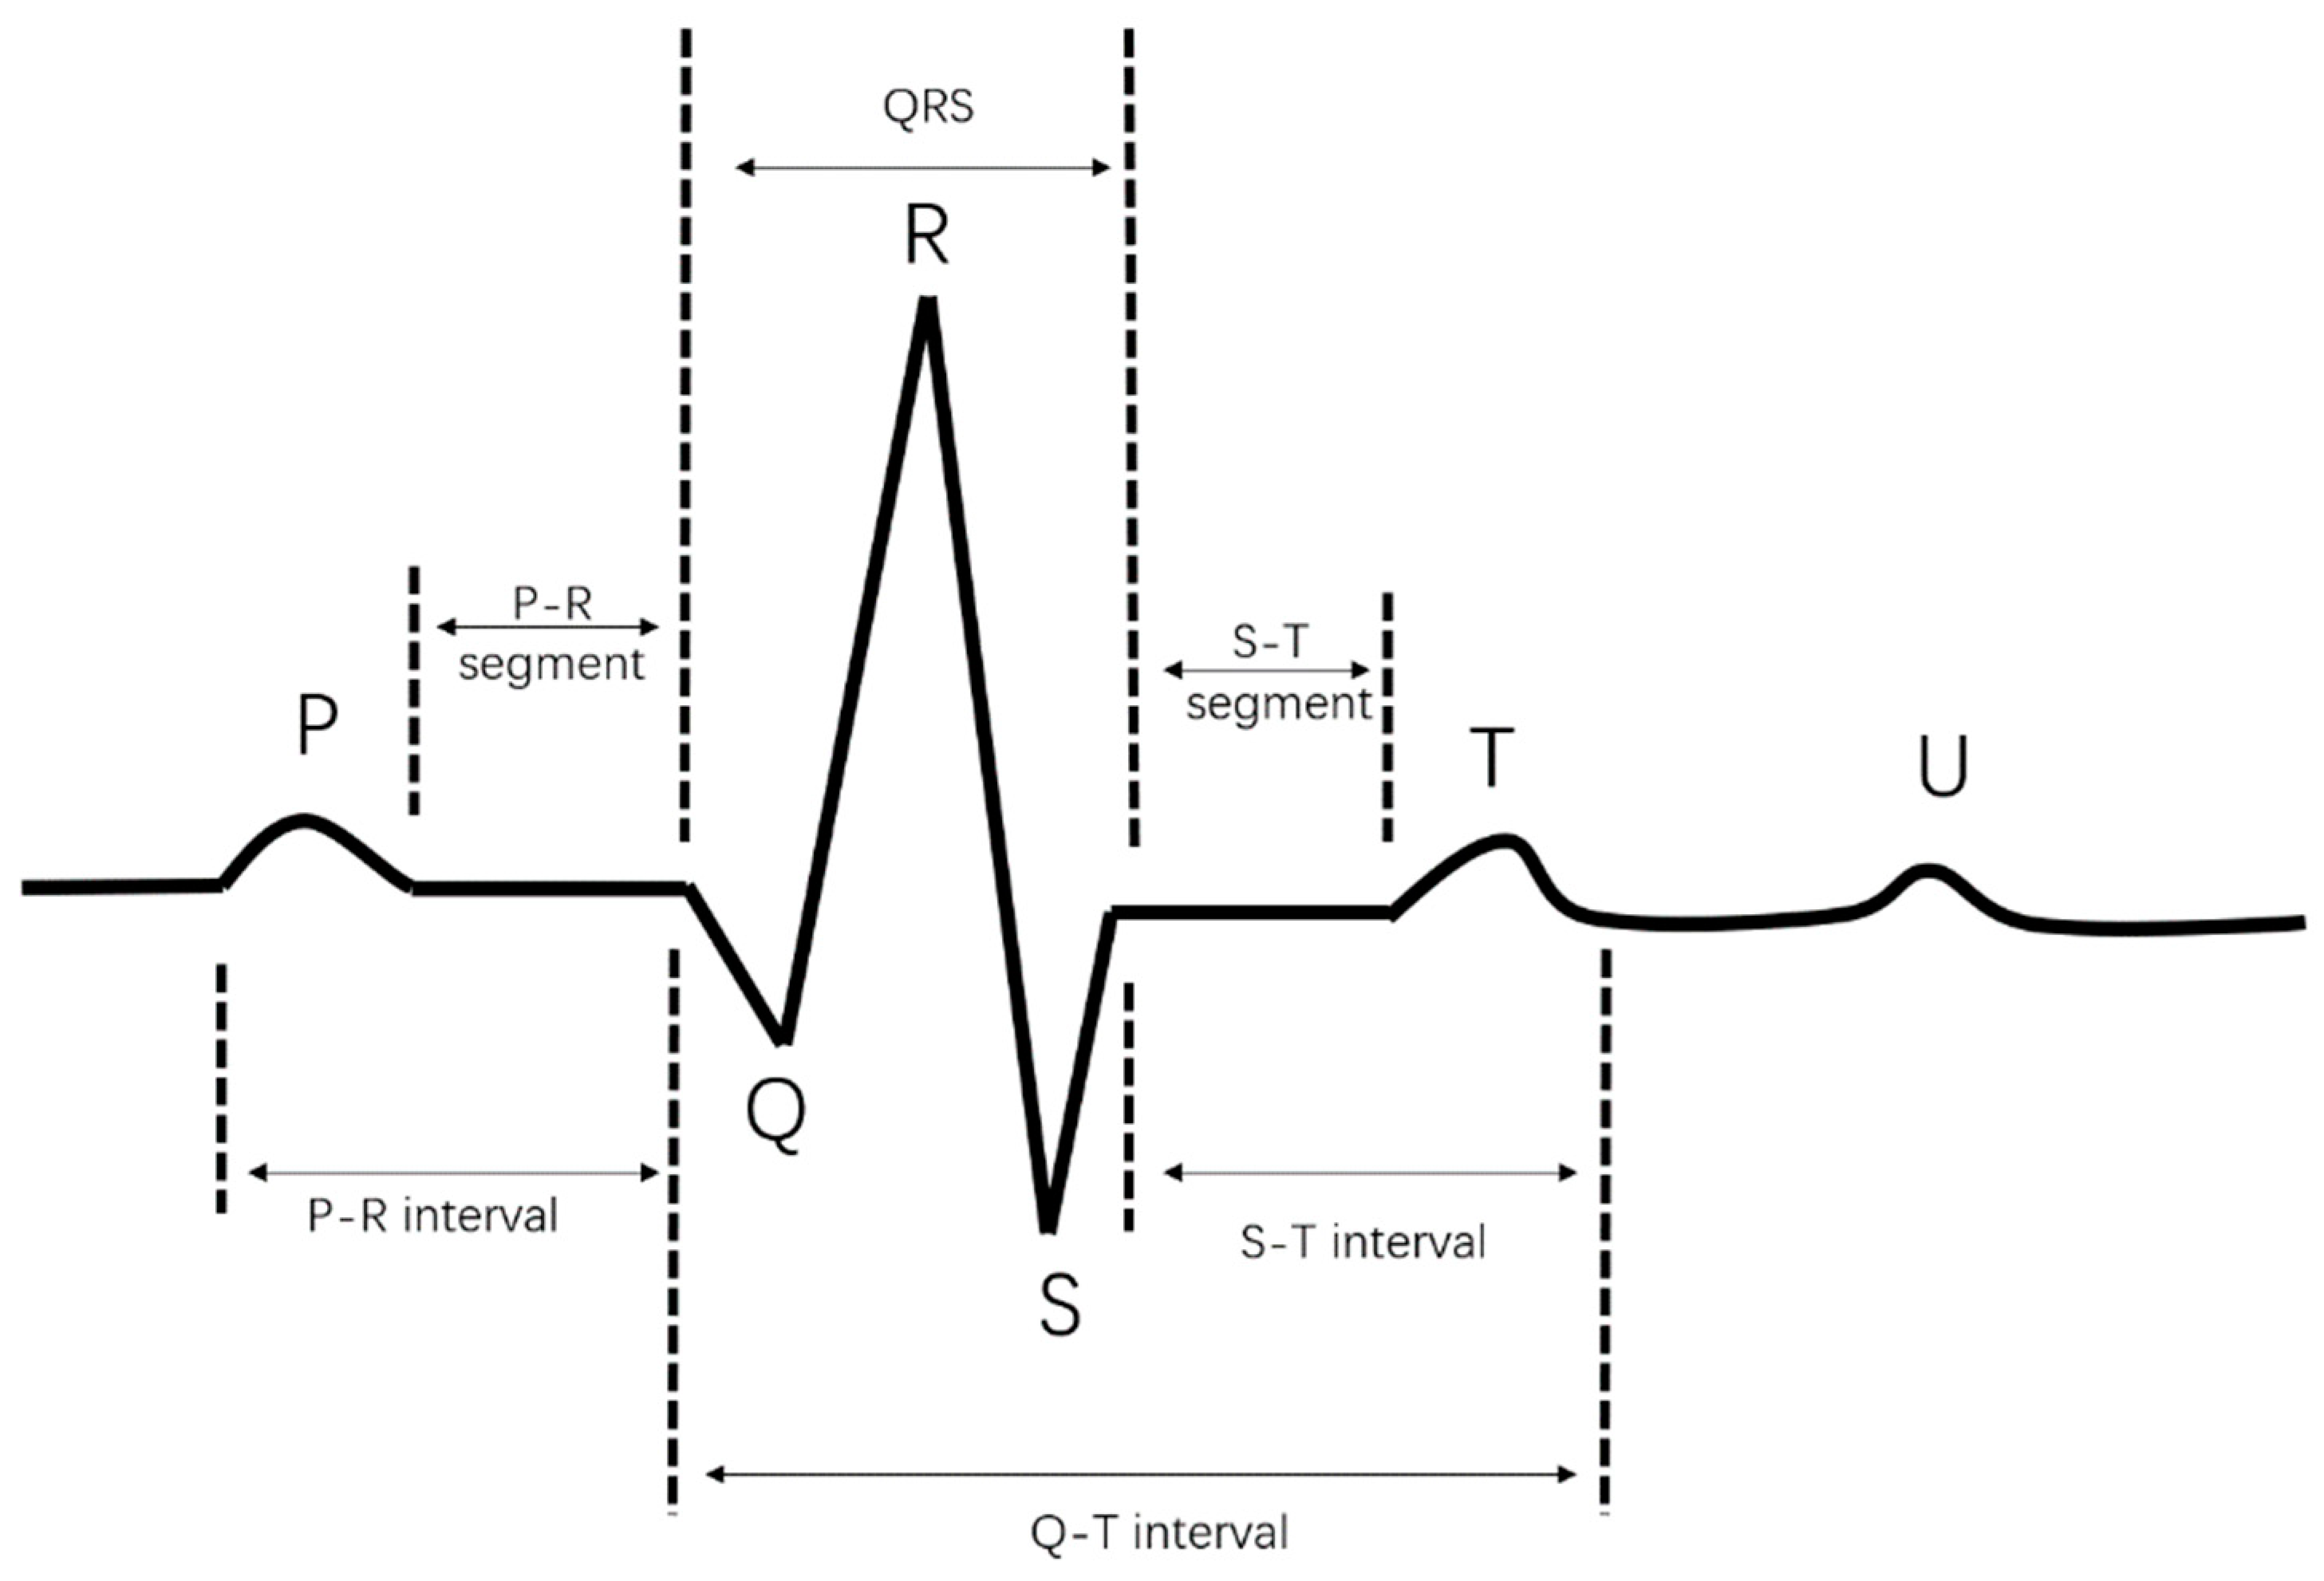
\includegraphics[width=0.8\textwidth]{img/ECG_ondas.png}
        \caption[Ciclo completo de un electrocardiograma]{Ciclo completo de un electrocardiograma\footnotemark}
        \label{fig:ECG_ondas}
    \end{figure}
    \footnotetext{Muestra el ciclo completo de un electrocardiograma, con las ondas P, Q, R, S, T y U, y los intervalos PR, QRS, ST y QT. Imagen tomada de encyclopedia.pub. [En línea]. Disponible en: \url{https://encyclopedia.pub/entry/52174}}

    El ECG tiene las características de baja frecuencia y concentración de energía, y la señal es débil, fácilmente perturbada por el ruido, como interferencias eléctricas, campos electromagnéticos externos, movimiento de electrodos (ruido instantáneo)  y el desplazamiento de la línea de base que es causado principalmente por la respiración. Estos ruidos dificultan el diagnóstico médico y pueden provocar errores en la identificación de enfermedades. Por ello, es esencial aplicar técnicas adecuadas para eliminar el ruido y mejorar la calidad de los datos de ECG muestreados \cite{AlMahamdy_2014}.

    \subsection{Fotopletismografía (PPG)}
        \subsubsection{Principios de la fotopletismografía}
            La fotopletismografía (PPG, por sus siglas en inglés) es una técnica óptica que puede utilizarse para detectar cambios en el volumen sanguíneo \cite{Hertzman_1938}. Un PPG es un dispositivo simple que consta de una fuente de luz y un detector; se han desarrollado dispositivos PPG que utilizan luz de diferentes longitudes de onda e intensidades basadas en la tecnología de diodos emisores de luz (LED). La cantidad de energía transferida a la piel por la luz depende de su longitud de onda; por ejemplo, la luz verde se utiliza con frecuencia y tiene una buena relación señal-ruido \cite{Challoner_1979}. Además, las señales de luz roja, verde y azul (RGB) permiten determinar el pulso y las frecuencias respiratorias.

            La función del fotodetector es detectar y cuantificar la luz absorbida durante el flujo pulsátil y no pulsátil. Durante el flujo pulsátil, la luz se absorbe por el cambio en el flujo sanguíneo dentro de las arterias, que es sincrónico con un latido del corazón. Durante el flujo no pulsátil, la luz se absorbe por los tejidos de fondo. Por lo tanto, un fotodetector detecta el cambio volumétrico en el flujo sanguíneo en las arterias al detectar la diferencia de intensidad de luz. La medición de este cambio en la intensidad de la luz ayuda a analizar la funcionalidad del corazón.

            En los últimos treinta años, el número de artículos publicados sobre PPG ha aumentado significativamente, abarcando tanto la investigación básica como la aplicada. En todas estas publicaciones, la PPG ha sido elogiada como una técnica óptica no invasiva, de bajo costo y simple para medir parámetros fisiológicos aplicados en la superficie de la piel. \cite{PPG}.

            La popularidad de este tema se puede atribuir a la comprensión de que la PPG tiene implicaciones importantes para una amplia gama de aplicaciones. Entre muchas, ayuda en la detección de oxígeno en sangre, la evaluación cardiovascular y el control de los signos vitales. Además, la importante contribución de la PPG en los dispositivos portátiles ha elevado exponencialmente la popularidad y la facilidad de uso de la PPG \cite{allen_2007}.

        \subsubsection{Modos de medición}
            La tecnología PPG mide los cambios en el volumen de sangre en los tejidos durante un ciclo cardíaco mediante una fuente de luz. Esta medición volumétrica proporciona información importante sobre el sistema cardiovascular. Un sensor PPG consta principalmente de dos componentes electrónicos: un emisor de luz y un detector de intensidad lumínica.

            Generalmente, se utiliza un LED como emisor de luz y un fotodetector para captar los cambios en la intensidad lumínica. Un pulso PPG correspondiente a un latido del corazón que incluye las fases sistólica y diastólica. Durante la fase sistólica, el corazón se contrae y empuja la sangre rica en oxígeno hacia los tejidos y órganos, lo que incrementa el volumen de sangre en las arterias. Esto provoca que las células sanguíneas absorban más luz, por lo que la cantidad de luz detectada por el fotodetector es menor. En cambio, durante la fase diastólica, el corazón se relaja y la sangre regresa a él, disminuyendo el volumen sanguíneo en las arterias, como resultado, se absorbe menos luz y el fotodetector registra un aumento en la intensidad lumínica.\cite{Hiiberia_2023}.

            Dependiendo de la aplicación y la ubicación del sensor, el PPG se puede usar en modo transmisivo o en modo de reflexión.

            \begin{enumerate}
                \item [a] Cuando un fotodetector y un LED se colocan en lados opuestos de un dedo para detectar la luz transmitida, este arreglo se conoce como modo transmisivo. En este modo, la sonda está configurada de manera que el fotodetector y el LED se enfrentan con una capa de tejido entre ellos. La detección en modo transmisivo depende de la luz que atraviesa las partes del cuerpo, por lo que se prefieren estructuras delgadas como el lóbulo de la oreja y el dedo.
                \item [b] Cuando el fotodetector y el LED se colocan en el mismo lado de un dedo para detectar la luz reflejada, se utiliza el modo reflectivo. En este arreglo, ambos sensores se sitúan uno al lado del otro con una pequeña separación. Por lo tanto, el modo reflectivo puede emplearse en cualquier parte del cuerpo, como la frente o la muñeca.
            \end{enumerate}

            \begin{figure}[H]
                \centering
                \begin{subfigure}[b]{0.45\linewidth}
                    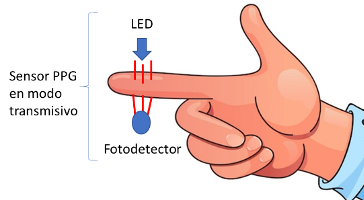
\includegraphics[width=\linewidth]{img/PPG_transmisivo.png}
                    \caption{Sensor PPG en modo de transmisión}
                    \label{fig:PPG_transmisivo}
                \end{subfigure}
                \begin{subfigure}[b]{0.45\linewidth}
                    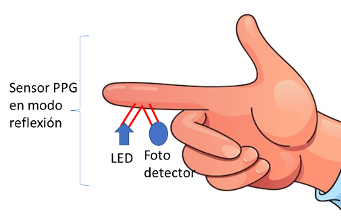
\includegraphics[width=\linewidth]{img/PPG_reflexion.png}
                    \caption{Sensor PPG en modo de reflexión}
                    \label{fig:PPG_reflexion}
                \end{subfigure}
                \caption[Modos de medición de la fotopletismografía]{Modos de medición de la fotopletismografía\footnotemark}
                \label{fig:modosMedicionPPG}
            \end{figure}
            \footnotetext{Muestra la posición de los sensores PPG en modo de transmisión y en modo de reflexión, los dos modo se utiliza para medir la fotopletismografía. Imagen tomada de aiva.hi. [En línea]. Disponible en: \url{https://goo.su/pg8UGx}}

            \subsubsection{Forma de onda de un PPG}

            En la figura \ref{fig:PPG} se muestra la señal característica de un fotopletismógrado, la cual está directamente relacionada con la frecuencia cardíaca, donde cada periodo de la señal corresponde a una pulsación del corazon.

            La señal representa dos picos por cada periodo, el pico mayor representa la presión sistólica, y el segundo pico representa el inicio de la presión diastólica cuyo valor es el mínimo de la curva \cite{Celi_2011}.

            Para calcular la frecuencia cardíaca (FC) a partir de la señal PPG, se utiliza la ecuación~\ref{eq:FrecienciaCardiaca}, donde el intervalo entre pico a pico es el tiempo transcurrido entre dos pulsaciones del corazón.

            \begin{equation}
                \label{eq:FrecienciaCardiaca}
                FC = \frac{60}{\textit{Intervalo entre picos}}
            \end{equation}

            \begin{figure}[H]
                \centering
                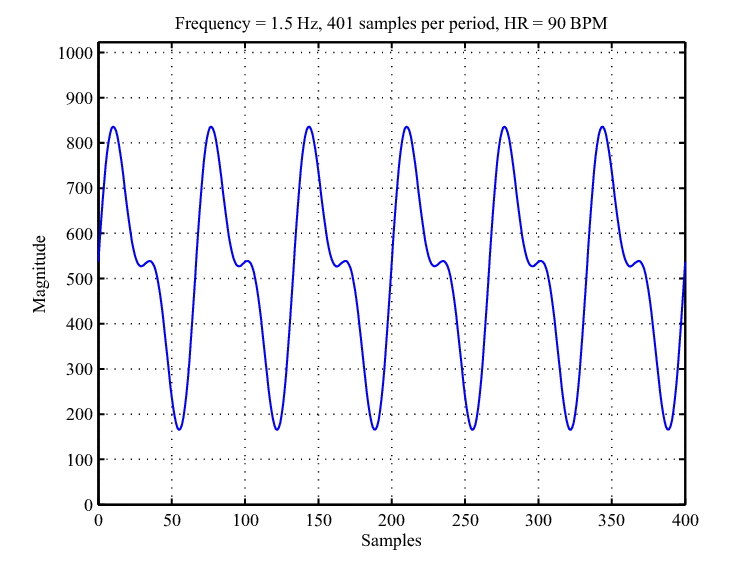
\includegraphics[width=0.7\textwidth]{img/PPG_senial.png}
                \caption[Modelo matemático de una señal pura de una fotopletismografía]{Modelo matemático de una señal pura de una fotopletismografía\footnotemark}
                \label{fig:PPG}
            \end{figure}
            \footnotetext{Muestra una representación de una señal pura de una fotopletismografía, donde se observa la forma de onda de la señal con una frecuencia de 1.5 Hz, que representa 90 latidos por minuto. Imagen tomada del articulo ``Body sensor network for mobile health monitoring, a diagnosis and anticipating system´´. [En línea]. Disponible en: \url{https://doi.org/10.1109/jsen.2015.2464773}}

        
        \subsubsection{Componente AC y DC de la señal PPG}
            La figura \ref{fig:PPG_AC_DC} muestra un ejemplo de una forma de onda fotopletismográfica, que tiene componentes de corriente continua (DC) y corriente alterna (AC). El componente DC de la forma de onda PPG corresponde a la señal óptica transmitida o reflejada del tejido y depende de la estructura del tejido y del volumen promedio de la sangre arterial y venosa. El componente DC cambia lentamente con la respiración, mientras que el componente AC fluctúa de acuerdo con los cambios en el volumen sanguíneo que ocurren entre las fases sistólica y diastólica del ciclo cardíaco \cite{Tamura_2019}.

            Cuando el corazón bombea sangre durante la sístole, el aumento del volumen sanguíneo en los tejidos periféricos provoca una mayor absorción de la luz o una menor reflexión, lo que da lugar a una desviación hacia abajo en la forma de onda PPG. Durante la diástole, cuando el corazón se relaja, el volumen sanguíneo disminuye, lo que da lugar a una desviación hacia arriba en la forma de onda PPG. La tecnología basada en PPG calcula las mediciones en función de los cambios reflejados en la forma de onda \cite{Cabessa_2024}.

            \begin{figure}[H]
                \centering
                \begin{subfigure}[b]{0.45\linewidth}
                    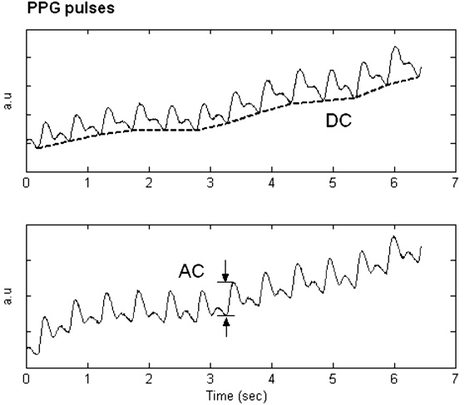
\includegraphics[width=\linewidth]{img/PPG_AC_DC.png}
                \end{subfigure}
                \begin{subfigure}[b]{0.45\linewidth}
                    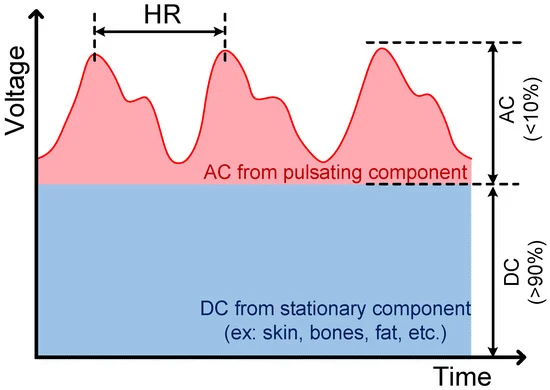
\includegraphics[width=\linewidth]{img/PPG_Componente_AC_DC.png}
                \end{subfigure}
                \caption[Componente AC y DC de la señal PPG]{Componente AC y DC de la señal PPG\footnotemark}
                \label{fig:PPG_AC_DC}
            \end{figure}
            \footnotetext{Muestra un ejemplo de forma de onda de la señal PPG, donde se observa el componente AC y DC de la señal. Imagen tomada del artículo ``Wearable Photoplethysmographic Sensors—Past and Present". [En línea]. Disponible en: \url{https://doi.org/10.3390/electronics3020282}}

        \subsubsection{Longitud de onda de la luz emitida}
            La piel del cuerpo está compuesta principalmente por tres capas de tejido: la epidermis, la dermis y la hipodermis. Debido a la absorción, solo las ondas de luz con una longitud de onda mayor pueden penetrar a través de todas ellas. La hemoglobina oxigenada absorbe la luz infrarrojo (NIR), mientras que la hemoglobina desoxigenada absorbe luz en la longitud de onda roja. Como resultado, los PPG que emplean LED y fotodetectores con longitudes de onda NIR y roja se utilizan comúnmente en el control clínico para calcular la concentración de hemoglobina.

            Sin embargo, el movimiento del paciente influye en la precisión de la medición y está relacionado con la longitud de onda de la luz utilizada. La luz de longitud de onda más larga, como el infrarrojo, se ve más afectada por el movimiento debido a que penetra profundamente en el tejido. Por otro lado, la luz de longitud de onda más corta (luz verde) generalmente está libre de los efectos del movimiento, ya que penetra menos en el tejido corporal. Por lo tanto, para mitigar el impacto del movimiento y la absorción de luz por los tejidos, se ha propuesto el uso de PPG basados en sensores ópticos de múltiples longitudes de onda para detectar variaciones en el flujo sanguíneo a diferentes profundidades de la piel. \cite{Hiiberia_2023}.

            \begin{figure}[H]
                \centering
                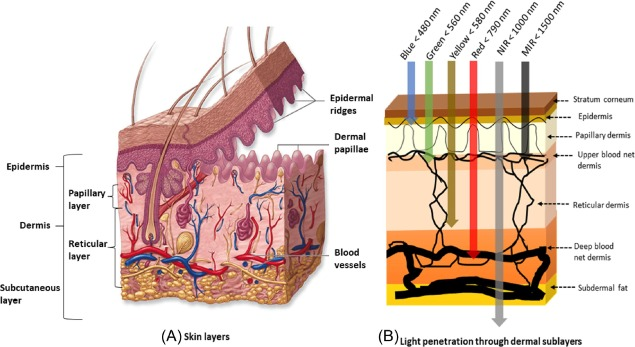
\includegraphics[width=0.8\textwidth]{img/PPG_luz.jpg}
                \caption[Penetración de las longitudes de onda de la luz en la piel]{Penetración de las longitudes de onda de la luz en la piel\footnotemark}
                \label{fig:PPG_longitud_onda}
            \end{figure}
            \footnotetext{Muestra la penetración de la luz en la piel, donde se observa que la luz de longitud de onda más larga (infrarroja) penetra más en la piel que la luz de longitud de onda más corta (Azul). Imagen tomada de Journal of Clinical Monitoring and Computing. [En línea]. Disponible en: \url{https://goo.su/jnUP8yi}}

            Dentro de la región visible, el pico de absorción dominante está en la región azul del espectro, seguido de la región verde-amarilla (500-600 nm), correspondiente a los glóbulos rojos. La luz de longitudes de onda más cortas es absorbida fuertemente por la melanina. El agua absorbe la luz en las regiones ultravioleta e infrarroja (IR) más largas. La luz roja (660 nm) e IR (940nm) pasa a través del tejido y la sangre. Por lo tanto, la luz IR se ha utilizado en sensores PPG.
        
            En la última década, la eficiencia de los LED ha aumentado y su voltaje directo ha disminuido, lo que resulta en un mayor número de lúmenes por watt. Gracias a la iluminación de alta potencia, la variación en el ciclo cardíaco entre las fases sistólica y diastólica es más pronunciada en la longitud de onda verde. Por ello, la luz verde se ha empleado en sensores PPG para medir la frecuencia cardíaca y la saturación de oxígeno en la sangre. \cite{Tamura_2019}.

    \subsection{Presión Arterial}
    La presión arterial es la fuerza que ejerce la sangre contra las paredes de las arterias. Se mide en milímetros de mercurio (mmHg) y se expresa mediante dos valores: la presión sistólica y la presión diastólica. Esta medición se realiza con un baumanómetro \cite{PresionArterialDefinicion}.

    La presión sistólica, se produce cuando el corazón se contrae, impulsando la sangre y aumentando la presión sobre las arterias. La presión diastólica, se registra durante la fase de relajación del corazón, cuando la presión sobre las arterias disminuye \cite{fernandez_presion}.
    
    Se considera que una presión arterial normal es de 120/80 mmHg. La hipertensión se define con valores de 140/90 mmHg o superiores, mientras que la hipotensión se establece en 90/60 mmHg o inferiores \cite{DOF}.

    \begin{figure}[H]
        \centering
        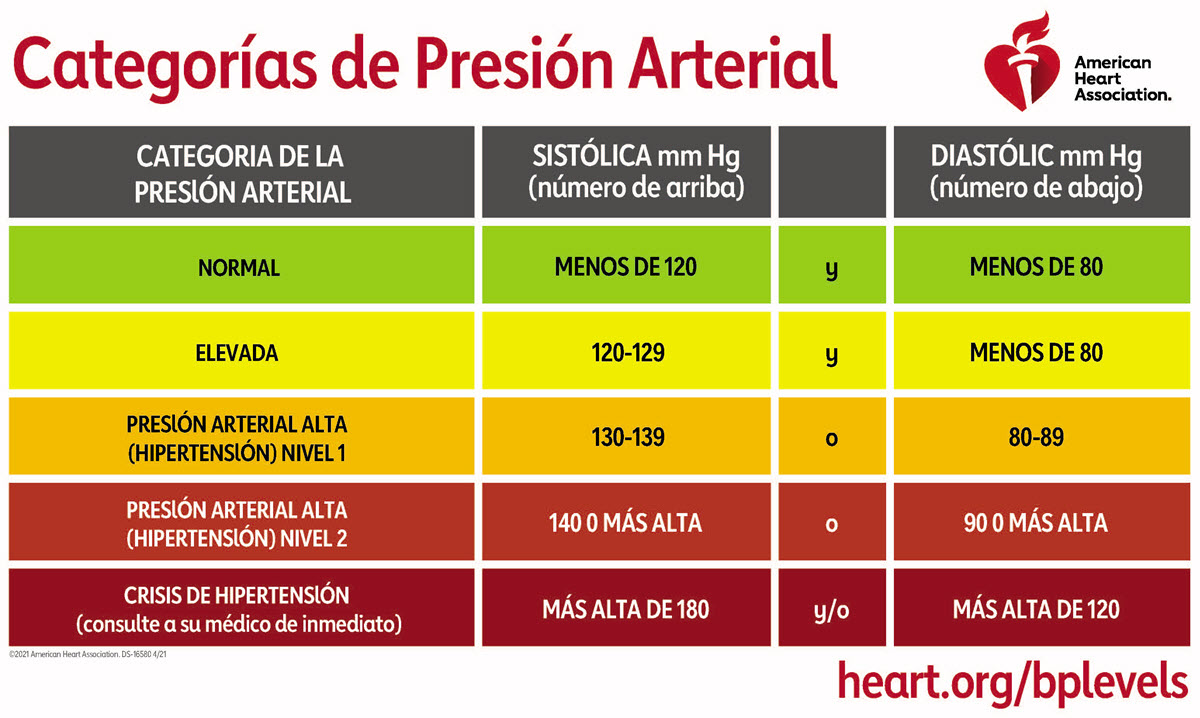
\includegraphics[width=0.8\textwidth]{img/Marco/PA_categoria.jpg}
        \caption[Cátegorias de la presión arterial]{Cátegorias de la presión arterial\footnotemark}
        \label{fig:PA_categoria}
    \end{figure}
    \footnotetext{Muestra las categorías de la presión arterial, donde se observa la presión arterial normal, elevada, hipertensión etapa 1, hipertensión etapa 2 y crisis hipertensiva. Imagen tomada de \textit{American Heart Association}. [En línea]. Disponible en: \url{https://goo.su/tBpC}}

    La hipertensión arterial, conocida como el ``asesino silencioso'' por ser asintomática en sus primeras etapas, suele pasar desapercibida hasta que se presentan complicaciones graves. Es la enfermedad de mayor prevalencia a nivel mundial y aumenta significativamente el riesgo cardiovascular. Un diagnóstico temprano, junto con el cumplimiento de las metas terapéuticas, es fundamental para reducir de forma importante el riesgo de complicaciones \cite{archivosCardiologia_2016}.

    \subsection{Amplificadores}
    La mayoría de las señales bioeléctricas del cuerpo humano son señales con una magnitud del orden de máximo $5 mV_{pp}$ y para poder ser registradas y analizadas, es necesario amplificarlas \cite{Diaz_amplificacion_señales}.

        \subsubsection{Amplificador operacional}
            Los amplificadores operacionales\footnote{``Introducción al amplificador operacional (OpAmp) - Amplificadores operacionales", Solución Ingenieril. [En línea]. Disponible en: \url{https://goo.su/zbbKl}} son dispositivos electrónicos que se utilizan para amplificar señales eléctricas. Estos dispositivos tienen dos entradas, una inversora y otra no inversora, y una salida. La salida del amplificador operacional es proporcional a la diferencia de voltaje entre las dos entradas multiplicada por un factor de ganancia. La ganancia de un amplificador operacional se puede ajustar mediante la selección de resistencias externas.

            \begin{figure}[H]
                \centering
                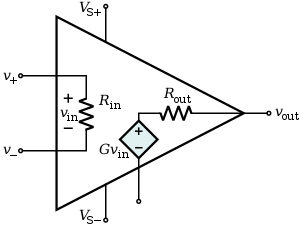
\includegraphics[width=0.5\textwidth]{img/Desarrollo/Amplificador_Operacional.png}
                \caption[Terminales de entrada y salida de un amplificador operacional]{Terminales de entrada y salida de un amplificador operacional\footnotemark}
                \label{fig:Amplificador_Operacional}
            \end{figure}
            \footnotetext{Muestra el símbolo electrónico de un amplificador operacional, con sus dos entradas, la ganancia de voltaje y la salida.}

            \begin{table}[H]
                \centering
                \begin{tabular}{ c | l }
                    Terminal & Descripción \\ \hline
                    $V_+$ & Entrada no inversora \\
                    $V_-$ & Entrada inversora \\
                    $V_{S+}$ & Alimentación positiva \\
                    $V_{S-}$ & Alimentación negativa \\
                    $V_{out}$ & Salida \\
                    $Gv_{in}$ & Ganancia de voltaje \\
                \end{tabular}
                \caption{Terminales del amplificador operacional}
                \label{tab:terminales_amplificador}
            \end{table}

        \subsubsection{Amplificador Inversor}
            El amplificador inversor \footnote{``Amplificador inversor - Amplificadores operacionales", Solución Ingenieril. [En línea]. Disponible en: \url{https://goo.su/eJTCVj}} es una configuración de amplificador operacional en la que la señal de entrada se aplica a la terminal inversora. En esta configuración, la salida está desfasada 180 grados con respecto a la entrada.

            El amplificador inversor se configura conectando la señal de entrada a la terminal inversora mediante una resistencia $R_i$. La salida del amplificador operacional retroalimenta a la terminal inversora a través de una resistencia $R_f$, como se muestra en la figura~\ref{fig:Amplificador_Inversor}.
            
            \begin{figure}[H]
                \centering
                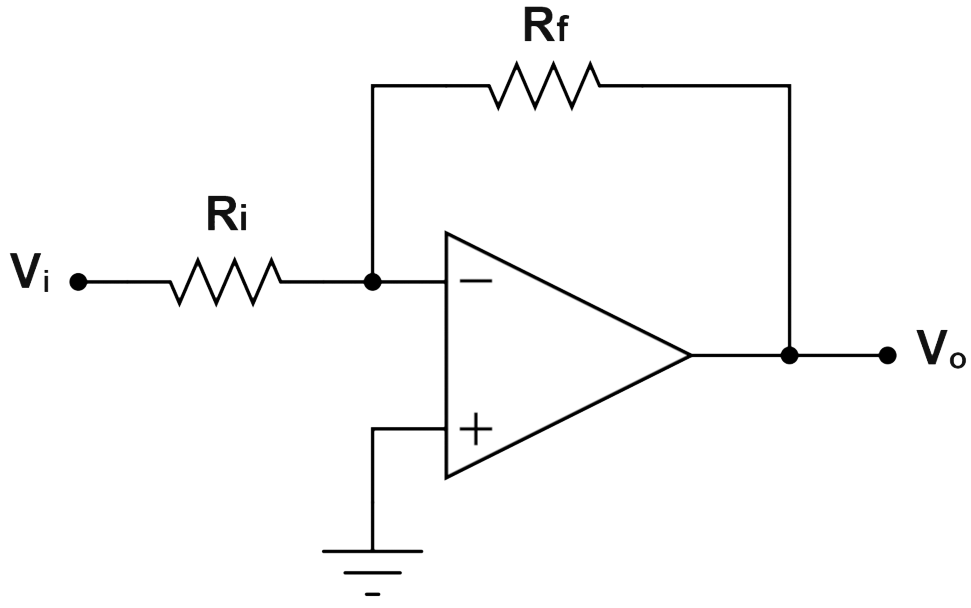
\includegraphics[width=0.5\textwidth]{img/Desarrollo/Amplificador_Inversor.png}
                \caption[Amplificador inversor]{Amplificador inversor\footnotemark}
                \label{fig:Amplificador_Inversor}
            \end{figure}
            \footnotetext{Muestra el diagrama esquemático de un amplificador inversor.}

            La ganancia del amplificador inversor se puede calcular mediante la ecuación~\ref{eq:ganancia_inversor}.

            \begin{equation}
                \label{eq:ganancia_inversor}
                G = -\frac{R_f}{R_i}
            \end{equation}

            Donde $G$ es la ganancia del amplificador, $R_f$ es la resistencia de retroalimentación y $R_i$ es la resistencia de entrada.

        \subsubsection{Amplificador No Inversor}
            El amplificador no inversor\footnote{``Amplificador No inversor - Amplificadores operacionales", Solución Ingenieril.[En línea]. Disponible en: \url{https://goo.su/8XuqHr}} es una configuración de amplificador operacional en la que la señal de entrada se aplica a la terminal no inversora. La salida de esta configuración está en fase con la entrada, y su amplitud es proporcional a la ganancia del amplificador.

            El amplificador no inversor se configura conectando la señal de entrada a la terminal no inversora, esto nos indica que la ganancia será positiva (al contrario del inversor). La salida del amplificador operacional se retroalimenta a la terminal inversora a través de una resistencia $R_f$, como se muestra en la figura~\ref{fig:Amplificador_No_Inversor}.

            \begin{figure}[H]
                \centering
                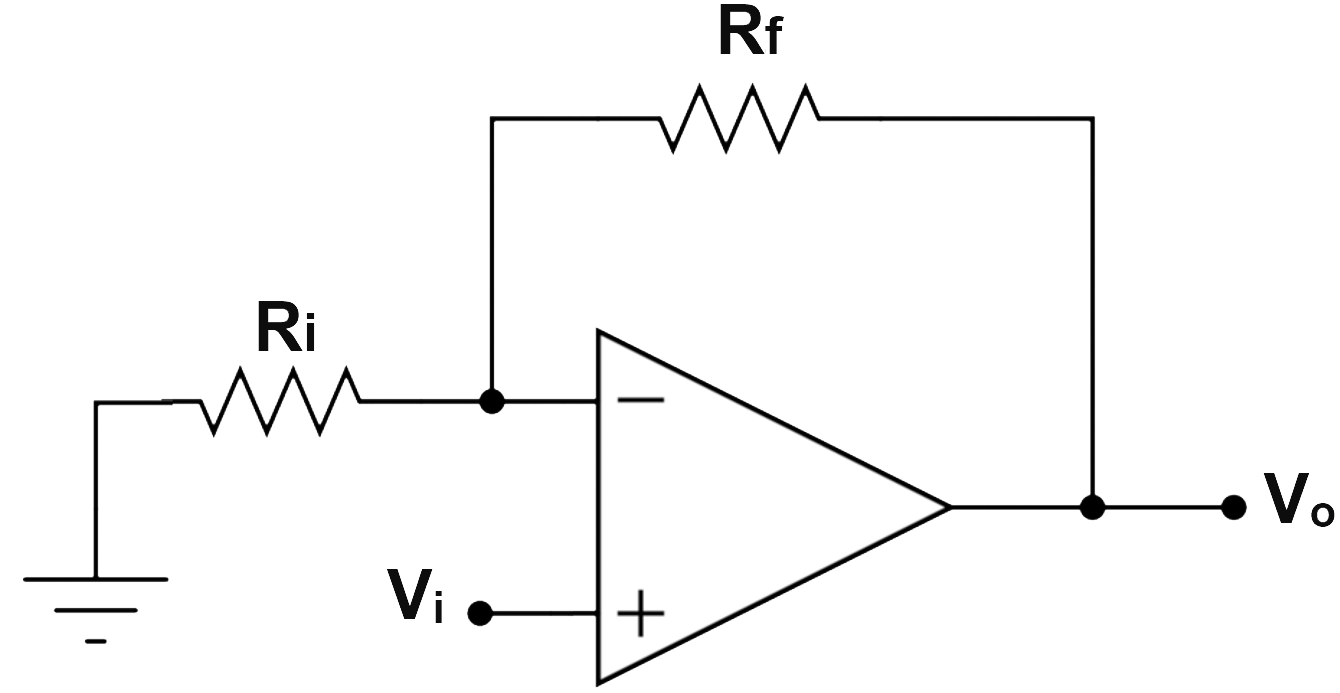
\includegraphics[width=0.5\textwidth]{img/Desarrollo/Amplificador_No_Inversor.png}
                \caption[Amplificador no inversor]{Amplificador no inversor\footnotemark}
                \label{fig:Amplificador_No_Inversor}
            \end{figure}
            \footnotetext{Muestra el diagrama esquemático de un amplificador no inversor.}

            La ganancia del amplificador no inversor se puede calcular mediante la ecuación~\ref{eq:ganancia_no_inversor}.

            \begin{equation}
                \label{eq:ganancia_no_inversor}
                G = \frac{R_f}{R_i} + 1
            \end{equation}

            Donde $G$ es la ganancia del amplificador, $R_f$ es la resistencia de retroalimentación y $R_i$ es la resistencia de entrada.

        \subsubsection{Amplificador Diferencial}
            El amplificador diferencial\footnote{W. Storr, ``Differential amplifier - the voltage subtractor," Basic Electronics Tutorials. [En línea]. Disponible en: \url{https://goo.su/vDsY3K}} es un tipo de amplificador operacional cuya característica principal radica en su capacidad de amplificar la diferencia de voltaje entre sus dos entradas mientras rechaza las señales comunes presentes en ambas (CMRR, por sus siglas en inglés). En la figura~\ref{fig:Amplificador_Diferencial} se muestra el diagrama esquemático de un amplificador diferencial.

            \begin{figure}[H]
                \centering
                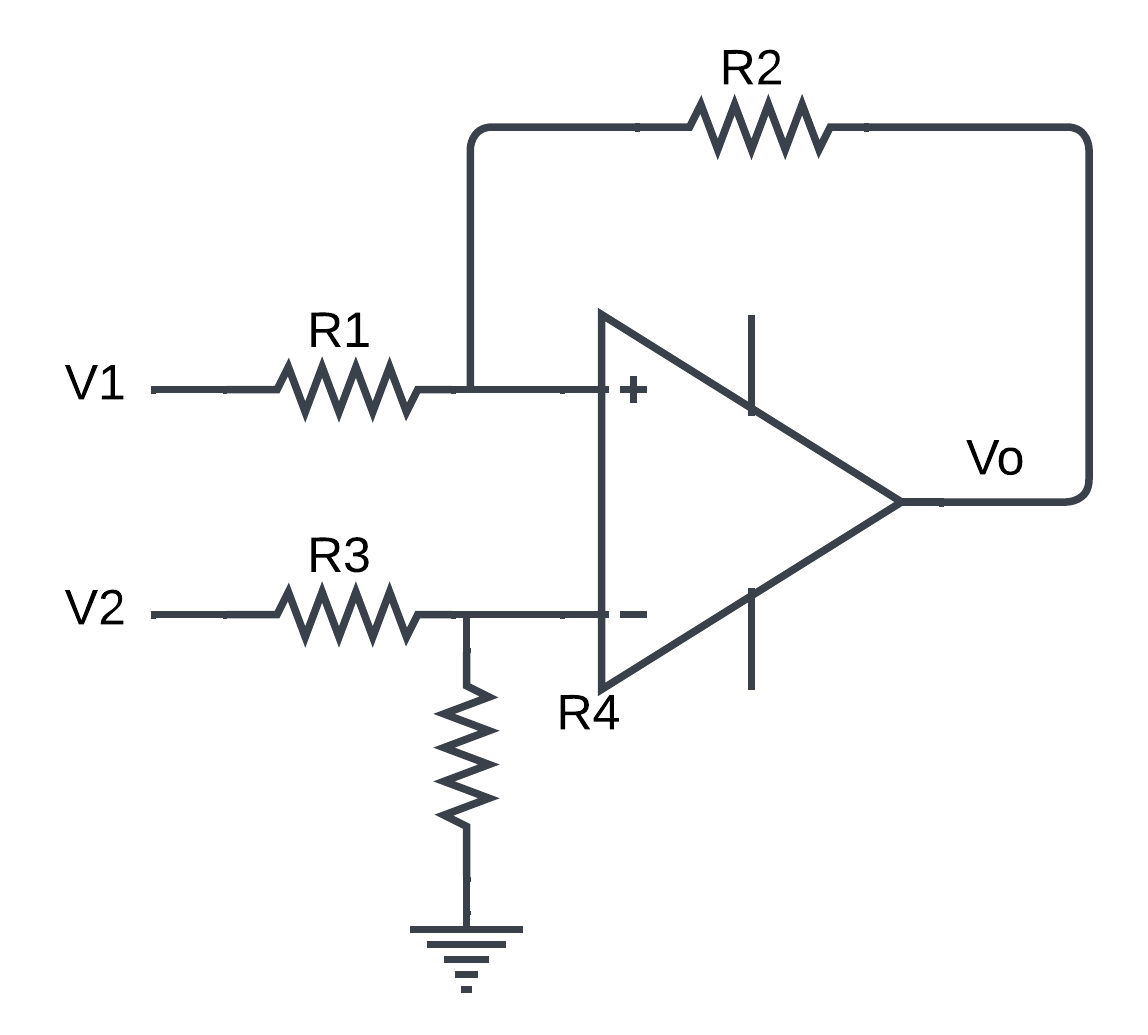
\includegraphics[width=0.5\textwidth]{img/Desarrollo/Amplificador_Diferencial.png}
                \caption[Amplificador diferencial]{Amplificador diferencial\footnotemark}
                \label{fig:Amplificador_Diferencial}
            \end{figure}
            \footnotetext{Muestra el diagrama esquemático de un amplificador diferencial, con una ganancia de $\frac{R2}{R1}$.}

            El voltaje de salida ($v_0$) está determinado por la ecuación~\ref{eq:voltaje_diferencial}.

            \begin{equation}
                \label{eq:voltaje_diferencial}
                v_0 = (1 + \frac{R2}{R1}) \cdot \frac{R3}{R3 + R4} \cdot v2 - \frac{R2}{R1} \cdot v1
            \end{equation}

            Para optimizar el rendimiento del amplificador, se suele implementar una configuración simétrica donde las resistencias cumplen la condición $R1 = R3$ y $R2 = R4$. De esta forma, la ecuación~\ref{eq:voltaje_diferencial} se simplifica a la ecuación~\ref{eq:voltaje_diferencial_simplificada}.

            \begin{equation}
                \label{eq:voltaje_diferencial_simplificada}
                v_0 = \frac{R2}{R1} \cdot (v2 - v1)
            \end{equation}

            La ganancia del amplificador diferencial se puede calcular mediante la ecuación~\ref{eq:ganancia_diferencial}.

            \begin{equation}
                \label{eq:ganancia_diferencial}
                G = \frac{R2}{R1}
            \end{equation}

        \subsubsection{Amplificador de Instrumentación}
            Para amplificar señales bioeléctricas, como las del ECG, se requieren dos características en un amplificador: la primera es que presente una alta impedancia en sus termminales de entrada (elimina posibles caídas de voltaje de la señal cardiaca que den como resultado la reducción o anulación de su amplitud), y la segunda es que solamente amplifique la diferencia de voltaje existente entre dichas terminales. 
            
            El amplificador que reúne las dos caracteríasticas mencionadas es el amplificador de instrumentación\footnote{``Práctica 4 - El amplificador de instrumentación básico'', Universidad Michoacana de San Nicolás de Hidalgo Facultad de Ingeniería Eléctrica. [En línea]. Disponible en: https://goo.su/n7zlBm}.

            Para hacer posible lo anterior, todos los amplificadores de instrumentación se basan en el diseño mostrado en la figura~\ref{fig:Amplificador_Instrumentacion} que tiene una etapa con amplificadores no inversores (brindan alta impedancia) y enseguida una etapa de amplificación diferencial (casi siempre unitaria) \cite{Diaz_amplificacion_señales}.

            La expresión para calcular la ganancia y el voltaje de un amplificador de instrumentación se muestra en la ecuación~\ref{eq:ganancia_amplificador_instrumentación}.

            \begin{equation}
                \label{eq:voltaje_amplificador_instrumentación}
                v_0 = (1 + \frac{2R1}{RG}) \cdot (v2 - v1)
            \end{equation}

            \begin{equation}
                \label{eq:ganancia_amplificador_instrumentación}
                G = 1 + \frac{2R1}{RG}
            \end{equation}

            \begin{figure} [H]
                \centering
                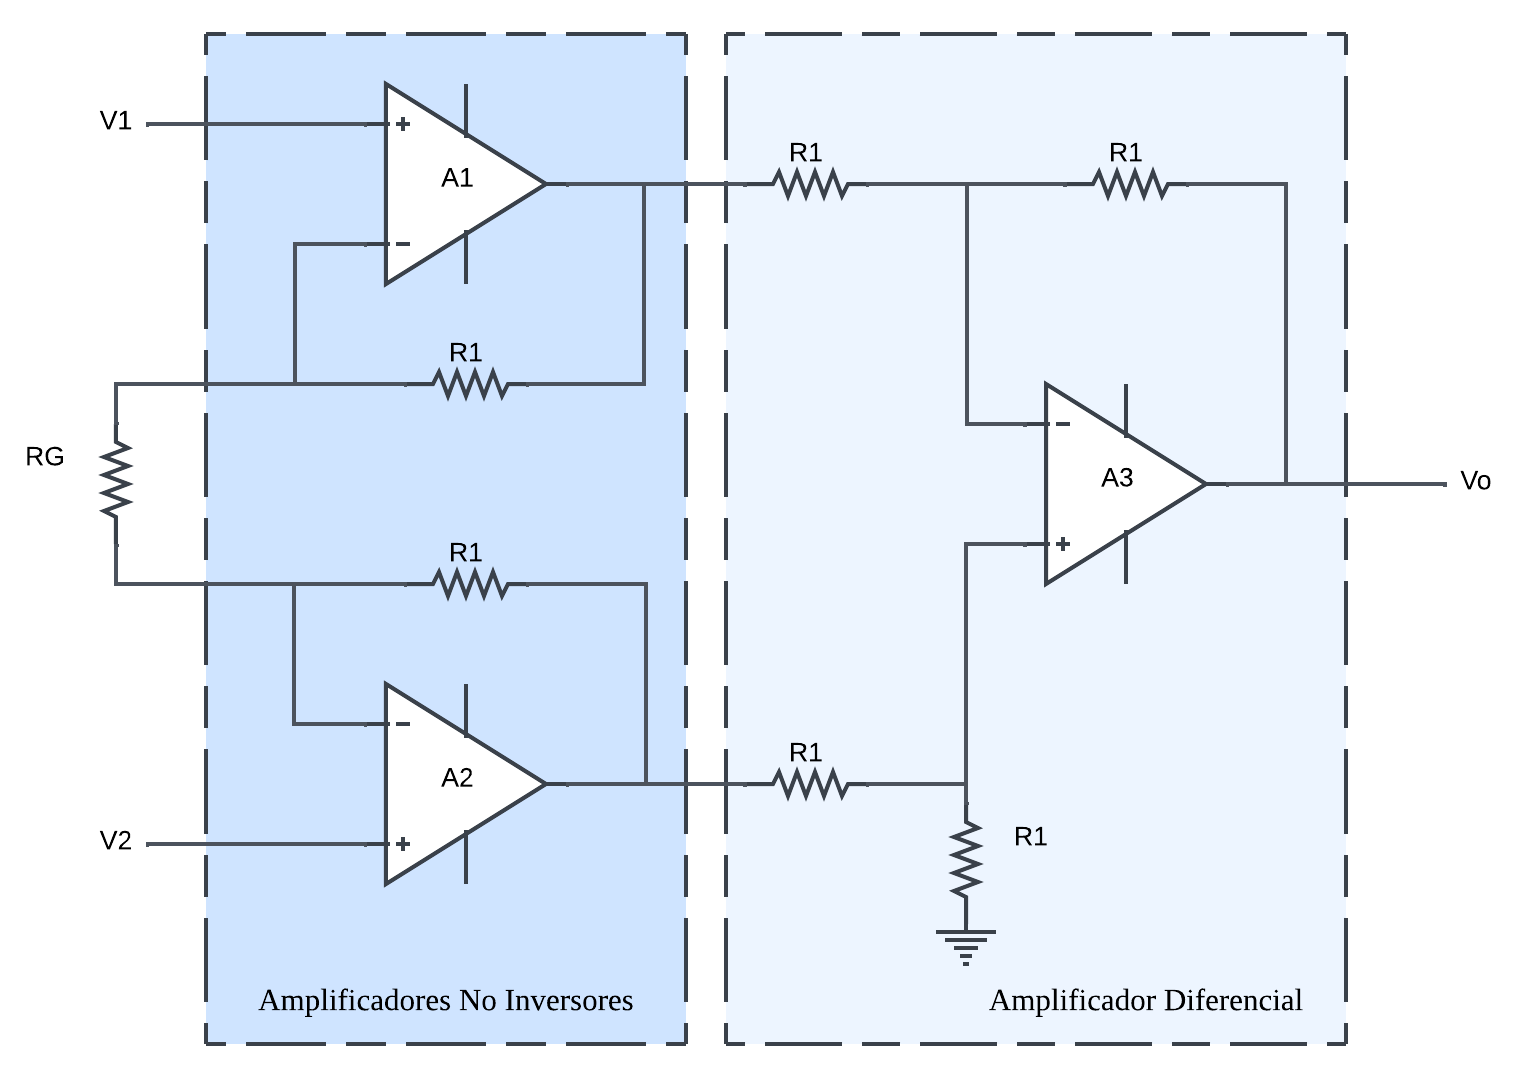
\includegraphics[width=0.5\textwidth]{img/Desarrollo/Amplificador_Intrumentacion.png}
                \caption[Amplificador de Instrumentación]{Amplificador de Instrumentación\footnotemark}
                \label{fig:Amplificador_Instrumentacion}
            \end{figure}
            \footnotetext{Diagrama de los elementos básicos que conforman las dos etapas en un amplificador de instrumentación. Imagen tomada de \textit{Fundamentals of operational amplifiers and linear integrated circuits}, p. 34.}

        \subsubsection{Amplificador de Intrumentación AD620}
            El amplificador de instrumentación AD620, es un amplificador de precisión de bajo costo y bajo consumo de energía fabricado por Analog Devices, que se utiliza para amplificar señales de baja amplitud y alta impedancia, como las señales ECG \cite{AD620_AnalogDevices,AD620_DigiKey}.

            \begin{figure}[H]
                \centering
                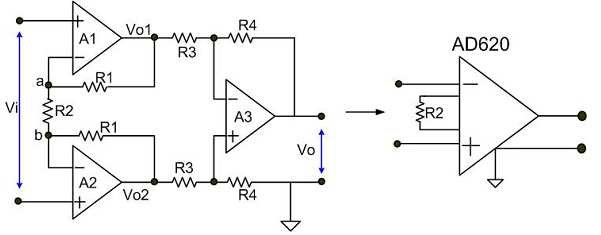
\includegraphics[width=0.8\textwidth]{img/Desarrollo/AD620.png}
                \caption[Diagrama esquemático del amplificador de instrumentos AD620.]{Diagrama esquemático del amplificador de instrumentos AD620\footnotemark}
                \label{fig:AD620}
            \end{figure}
            \footnotetext{Muestra que el amplificador de instrumentación AD620 es equivalente a un amplificador diferencial conectado a dos amplificadores no inversores. Imagen tomada del artículo \textit{Axial and Lateral Small Strain Measurement of Soils in Compression Test using Local Deformation Transducer} de la revista \textit{Journal of Engineering and Technological Sciences}. [En línea]. Disponible en: \url{https://goo.su/fHljmIK}}

            \hfill \break
            Características del AD620:
            \begin{itemize}
                \item \textbf{Ganancia configurable:} Ajustable de 1 a 10,000 mediante una resistencia externa.
                \item \textbf{Bajo Nivel de Ruido:} Minimiza errores en la señal amplificada, asegurando una representación precisa de la actividad eléctrica cardíaca.
                \item \textbf{Baja Corriente de Polarización de Entrada:} Con una tensión de polarización máxima de $50 \mu V$ y una deriva mínima de $0,6 \mu V / ^{\circ} C$.
                \item \textbf{Bajo Consumo de Potencia:} Consume un máximo de $1,3 mA$, adecuado para dispositivos portátiles o alimentados por batería.
                \item \textbf{Rango de Voltaje de Alimentación:} Funciona con voltajes de $\pm 2,3 V$ a $\pm 18 V$.
            \end{itemize}

            El AD620 es una gran alternativa al arreglo tradiccional de tres amplificadores operacionales, ya que ofrece una mayor precisión y estabilidad, y requiere menos componentes externos. 

            \begin{figure}[H]
                \centering
                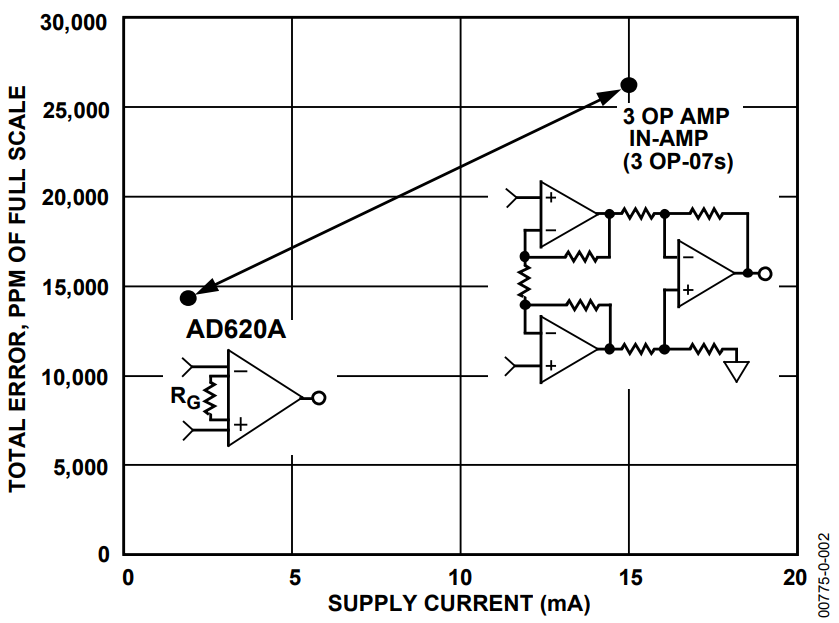
\includegraphics[width=0.6\textwidth]{img/Desarrollo/Amplificador_AD620_comparacion.png}
                \caption[Comparación de la taza de error entre el AD620 y un arreglo de amplificadores de instrumentación.]{Comparación de la taza de error entre el AD620 y un arreglo de amplificadores de instrumentación\footnotemark}
                \label{fig:Amplificador_AD620_comparacion}
            \end{figure}
            \footnotetext{Muestra la diferencia en la taza de error por corriente suministrada de un amplificador de instrumentación AD620 y un arreglo de amplificadores de instrumentación convencional. Imagen tomada del Datasheet del AD620. [En línea]. Disponible en: \url{https://goo.su/ZhlyZ}}

            El componente cuenta con una entrada inversora (pin 2), una no inversora (pin 3), dos fuentes de alimentación (pin 4 y 7), una referencia o polo a tierra (pin 5), y una salida de la señal amplificada (pin 6). La ganancia del AD620 se puede ajustar mediante una resistencia externa conectada entre el pin 1 y el pin 8.
            \begin{figure}[H]
                \centering
                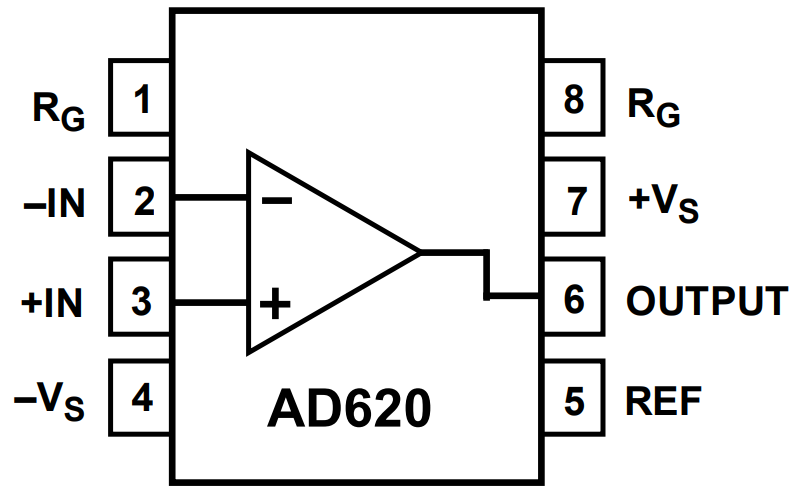
\includegraphics[width=0.6\textwidth]{img/Desarrollo/AD620_Diagrama.png}
                \caption[Esquema de conexión del amplificador de instrumentación AD620.]{Esquema de conexión del amplificador de instrumentación AD620\footnotemark}
                \label{fig:AD620_pinout}
            \end{figure}
            \footnotetext{Muestra el esquema de conexión del amplificador de instrumentación AD620, con sus terminales de alimentación, entrada y salida. Imagen tomada del Datasheet del AD620. [En línea]. Disponible en: \url{https://www.analog.com/media/en/technical-documentation/data-sheets/AD620.pdf}}

            Resulta que, en el marco de operación de este amplificador de instrumentación, es posible determinar la ganancia saliente a partir de la resistencia conectada entre los pines 1 y 8 \cite{AD620_AnalogDevices}, mediante la ecuación~\ref{eq:ganancia_AD620}.

            \begin{equation}
                \label{eq:ganancia_AD620}
                G = 1 + \frac{49.4 k\Omega}{R_G}
            \end{equation}

            Donde $G$ es la ganancia del amplificador, $R_G$ es la resistencia conectada entre los pines 1 y 8 y la constante $49.4 k\Omega$ es el valor de la resistencia interna del AD620.

    \subsection{Filtros}

        Los filtros son circuitos electrónicos que permiten el paso de ciertas frecuencias de una señal eléctrica, mientras que atenúan o eliminan las frecuencias no deseadas. Los filtros se utilizan para eliminar el ruido, mejorar la calidad de la señal y extraer información relevante de una señal eléctrica. Los filtros se pueden clasificar en dos categorías principales: filtros pasivos y filtros activos.

        \subsubsection{Filtro Pasa Altas Activo de Segundo Orden Sallen-Key}

            Un filtro pasa altos activo de segundo orden \textit{Sallen-Key}\footnote{W. Laiton, «Filtro Pasa altos activo de 2do orden Sallen Key», Wilaeba Electronica, 26 de septiembre de 2018. [En línea]. Disponible en: \url{https://goo.su/5ChsR5h}} es un circuito que permite el paso de señales de alta frecuencia y atenúa las frecuencias bajas. Este filtro consta de dos resistencias y dos capacitores, y se puede configurar para diferentes aproximaciones de filtro, como Butterworth, Chebyshev y Bessel. Se conoce como activo por que tiene un elemento activo que es el amplificador operacional, es de segundo orden por que contiene dos elementos reactivos (dos capacitores), y se llama sallen key por la topología que tiene el circuito, y por el nombre de sus dos creadores R. P. Sallen y E. L. Key, ingenieros del laboratorio Lincoln del MIT. La figura~\ref{fig:Filtro_Pasa_Altas} muestra el diagrama de un filtro pasa altas de segundo orden \textit{Sallen-Key}.

            \begin{figure}[H]
                \centering
                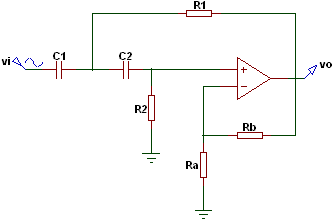
\includegraphics[width=0.6\textwidth]{img/Desarrollo/Filtro_Pasa_Altas.png}
                \caption[Diagrama de un filtro pasa altas de segundo orden \textit{Sallen-Key}.]{Diagrama de un filtro pasa altas de segundo orden \textit{Sallen-Key}}
                \label{fig:Filtro_Pasa_Altas}
            \end{figure}

            El valor de la frecuencia de corte $fc$, el valor del capacitor $C$ y la aproximación que se vaya a usar son libres de elección,  además de que la ganancia $A$ de este filtro debe ser igual o mayor a 1. La función de transferencia de un filtro pasa altas de segundo orden \textit{Sallen-Key} se puede calcular mediante la ecuación~\ref{eq:transferencia_pasaAltas}.

            \begin{equation}
                \label{eq:transferencia_pasaAltas}
                \frac{vo}{vi}(s) = \frac{(1 + \frac{R_b}{R_a})s^2}{s^2 + s\frac{1}{C}(\frac{2}{R_2} - \frac{R_b}{R_1R_a}) + \frac{1}{C^2R_1R_2}}
            \end{equation}

            Los valores de la constante $K$ y el factor de calidad $Q$ para diferentes aproximaciones de filtro se muestran en la tabla~\ref{tab:valores_filtro_pasa_altas}.
                
            \begin{table}[H]
                \centering
                \begin{tabular}{ l | c | c }
                    Aproximación & Factor de calidad $Q$ & Constante $K$ \\ \hline
                    Butterworth & 0.7071 & 1.0000 \\
                    Chebyshev (cresta de 0.01 db) & 0.7247 & 1.0231 \\
                    Chebyshev (cresta de 0.1 db) & 0.7673 & 1.0674 \\
                    Chebyshev (cresta de 0.25 db) & 0.8093 & 1.0991\\
                    Chebyshev (cresta de 0.5 db) & 0.8638 & 1.1286\\
                    Chebyshev (cresta de 1 db) & 0.9564 & 1.1596\\
                    Bessel & 0.5771 & 0.7840\\
                \end{tabular}
                \caption{Valores de $Q$ y $K$ para diferentes aproximaciones de filtro pasa altas}
                \label{tab:valores_filtro_pasa_altas}
            \end{table}

        \subsubsection{Filtro Pasa Bajas Activo de Segundo Orden Sallen-Key}

            Un filtro pasa bajas activo de segundo orden \textit{Sallen-Key}\footnote{W. Laiton, «Filtro Pasa bajas activo de 2do orden Sallen Key», Wilaeba Electronica, 24 de septiembre de 2018. [En línea]. Disponible en: \url{https://goo.su/J29uz5x}} es un circuito que permite el paso de señales de baja frecuencia y atenúa las frecuencias altas. Este filtro consta de dos resistencias y dos capacitores, y se puede configurar para diferentes aproximaciones de filtro, como Butterworth, Chebyshev y Bessel. La figura~\ref{fig:Filtro_Pasa_Bajas} muestra el diagrama de un filtro pasa bajas de segundo orden \textit{Sallen-Key}

            \begin{figure}[H]
                \centering
                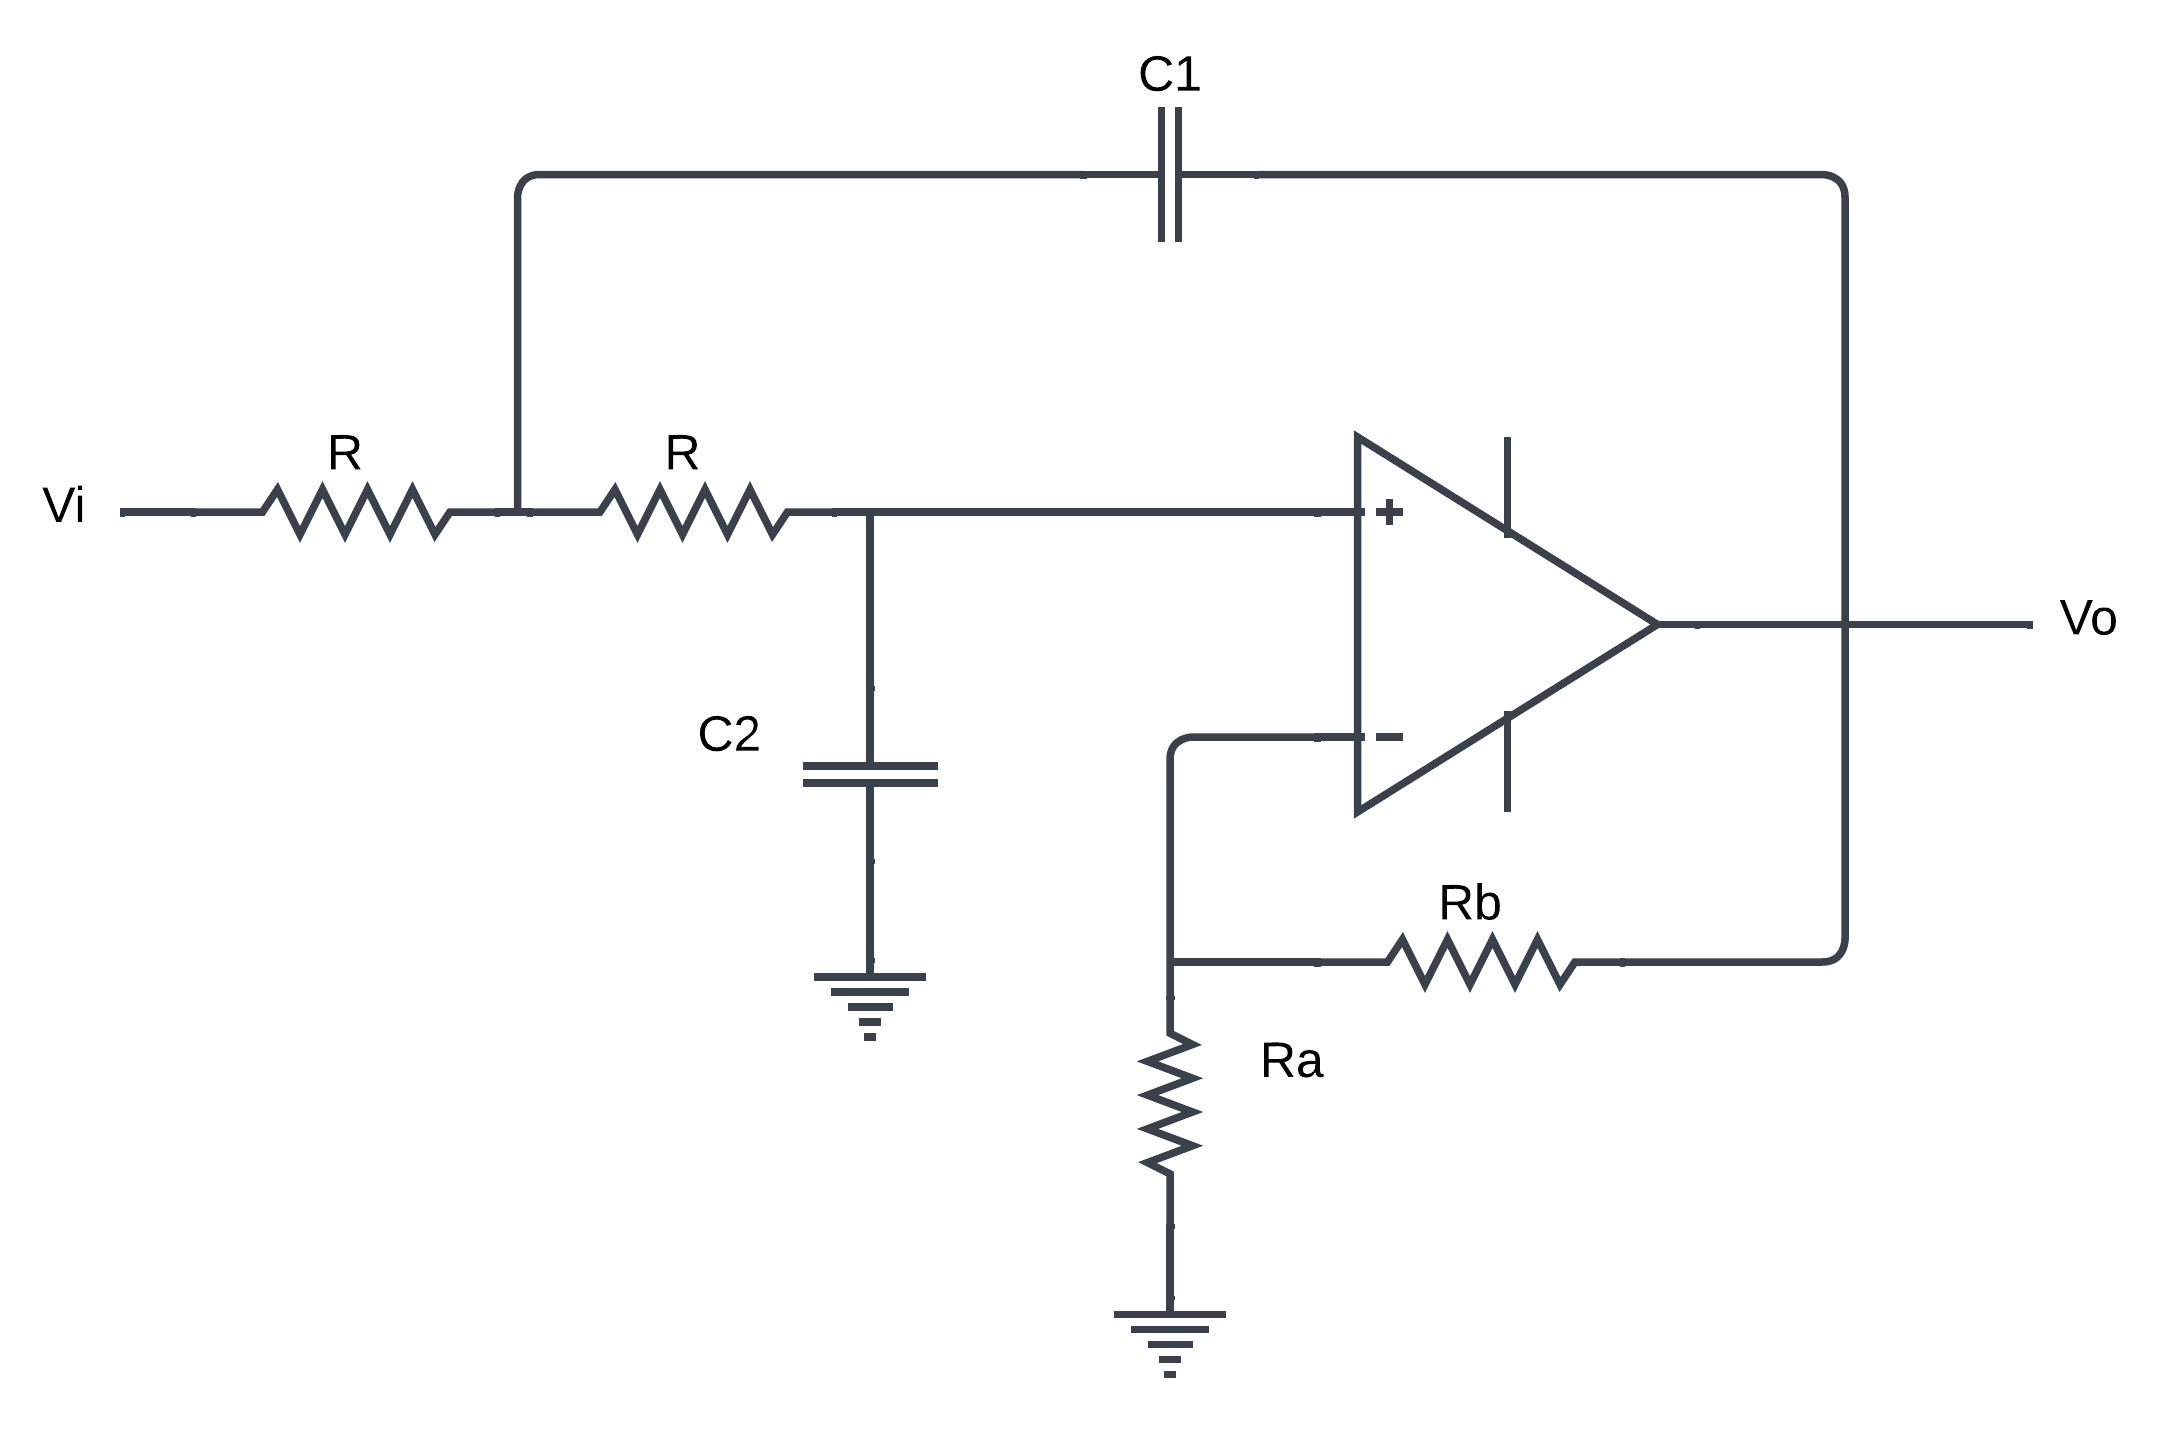
\includegraphics[width=0.6\textwidth]{img/Desarrollo/Filtro_pasa_bajas.png}
                \caption[Diagrama de un filtro pasa bajas de segundo orden \textit{Sallen-Key}.]{Diagrama de un filtro pasa bajas de segundo orden \textit{Sallen-Key}}
                \label{fig:Filtro_Pasa_Bajas}
            \end{figure}

            Los valores de la frecuencia de corte $f_c$, el capacitor $C_1$, y la aproximación que se desee utilizar son de libre elección. Además, la ganancia $A$ de este filtro debe ser igual o mayor a 1. La función de transferencia de un filtro pasa bajas de segundo orden \textit{Sallen-Key} se puede determinar utilizando la ecuación~\ref{eq:transferencia_pasaBajas}.

            \begin{equation}
                \label{eq:transferencia_pasaBajas}
                \frac{vo}{vi}(s) = \frac{(1+\frac{R_b}{R_a}) \cdot \frac{1}{C_1C_2R^2}}{s^2 + s\frac{1}{R}(\frac{2}{C_1} - \frac{R_b}{C_2R_a}) + \frac{1}{C_1C_2R^2}}
            \end{equation}

            Los valores de la constante $K$ y el factor de calidad $Q$ para diferentes aproximaciones de filtro se muestran en la tabla~\ref{tab:valores_filtro_pasa_bajas}.

            \begin{table}[H]
                \centering
                \begin{tabular}{ l | c | c }
                    Aproximación & Factor de calidad $Q$ & Constante $K$ \\ \hline
                    Butterworth & 0.7071 & 1.0000 \\
                    Chebyshev (cresta de 0.01 db) & 0.7247 & 0.9774 \\
                    Chebyshev (cresta de 0.1 db) & 0.7673 & 0.9368 \\
                    Chebyshev (cresta de 0.25 db) & 0.8093 & 0.9098\\
                    Chebyshev (cresta de 0.5 db) & 0.8638 & 0.8860\\
                    Chebyshev (cresta de 1 db) & 0.9564 & 0.8623\\
                    Bessel & 0.5771 & 1.2754\\
                \end{tabular}
                \caption{Valores de $Q$ y $K$ para diferentes aproximaciones de filtro pasa bajas}
                \label{tab:valores_filtro_pasa_bajas}
            \end{table}

        \subsubsection{Filtro Rechaza Banda Pasivo RC Twin-T}

            Un filtro rechaza banda (Notch) pasivo RC Twin-T\footnote{W. Laiton, «Filtro Rechaza banda Pasivo RC Twin-T», Wilaeba Electronica, 28 de septiembre de 2018. [En línea]. Disponible en: \url{https://goo.su/mTgR92}} como su nombre lo dice elimina una determinada banda de frecuencias, y permite el paso de todas las demás. Está compuesto por seis elementos, tres resistencias y tres capacitores. La figura~\ref{fig:Filtro_Rechaza_Banda} muestra el diagrama de un filtro rechaza banda pasivo RC Twin-T.

            \begin{figure}[H]
                \centering
                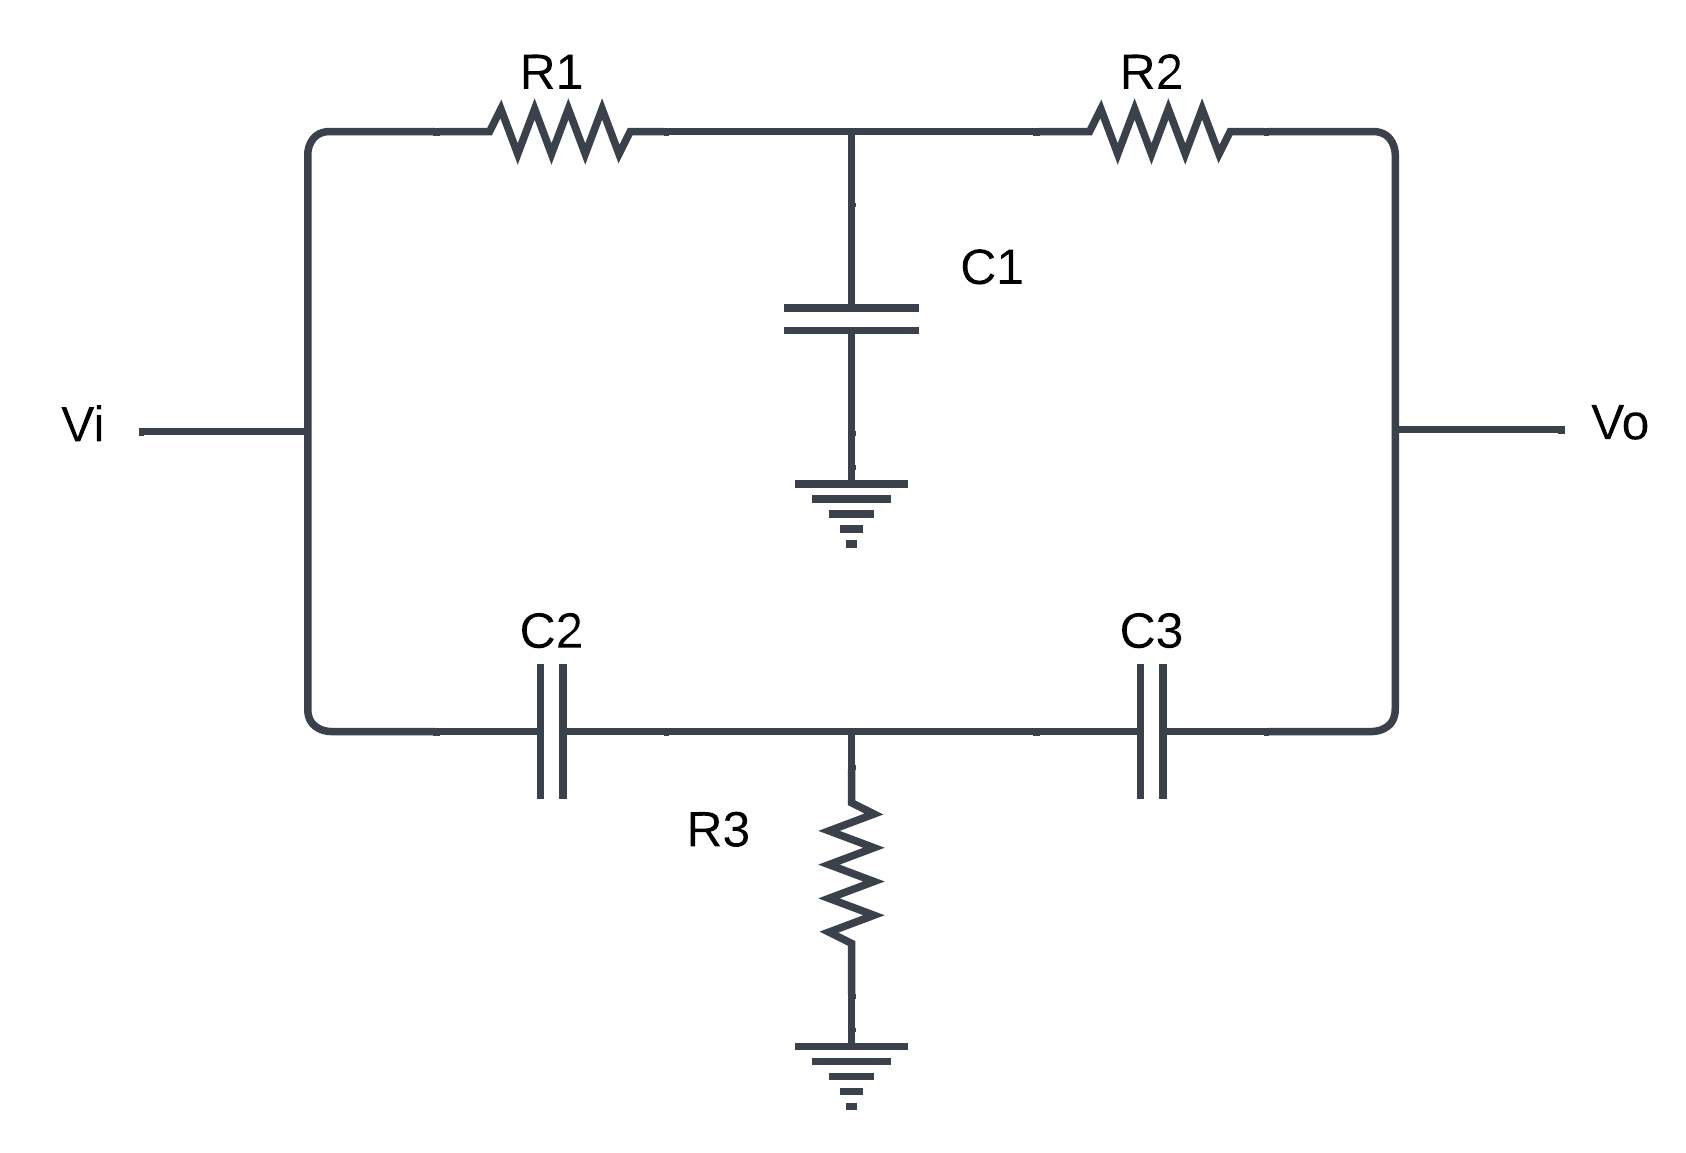
\includegraphics[width=0.6\textwidth]{img/Desarrollo/Filtro_Rechaza_Banda.png}
                \caption[Diagrama de un filtro rechaza banda pasivo RC Twin-T.]{Diagrama de un filtro rechaza banda pasivo RC Twin-T}
                \label{fig:Filtro_Rechaza_Banda}
            \end{figure}

            El máximo valor del factor de calidad $Q$ para un filtro rechaza banda pasivo RC Twin-T es de 0.5. Este filtro se conoce con el nombre de filtro notch Twin-T debido que son dos redes en forma de T conectadas en paralelo.
        

\newpage
\section{Desarrollo del Proyecto}
    \subsection{Flujo de operación del sistema}
    El sistema desarrollado cosnta de varios componentes que interactúan entre sí para capturar, procesar y transmitir datos fisiológicos, permitiendo al usuario visualizar información en tiempo real y estimar la presión arterial. El flujo de operación del sistema se muestra en la figura~\ref{fig:Flujo_Operacion}.

    \begin{figure}[H]
        \centering
        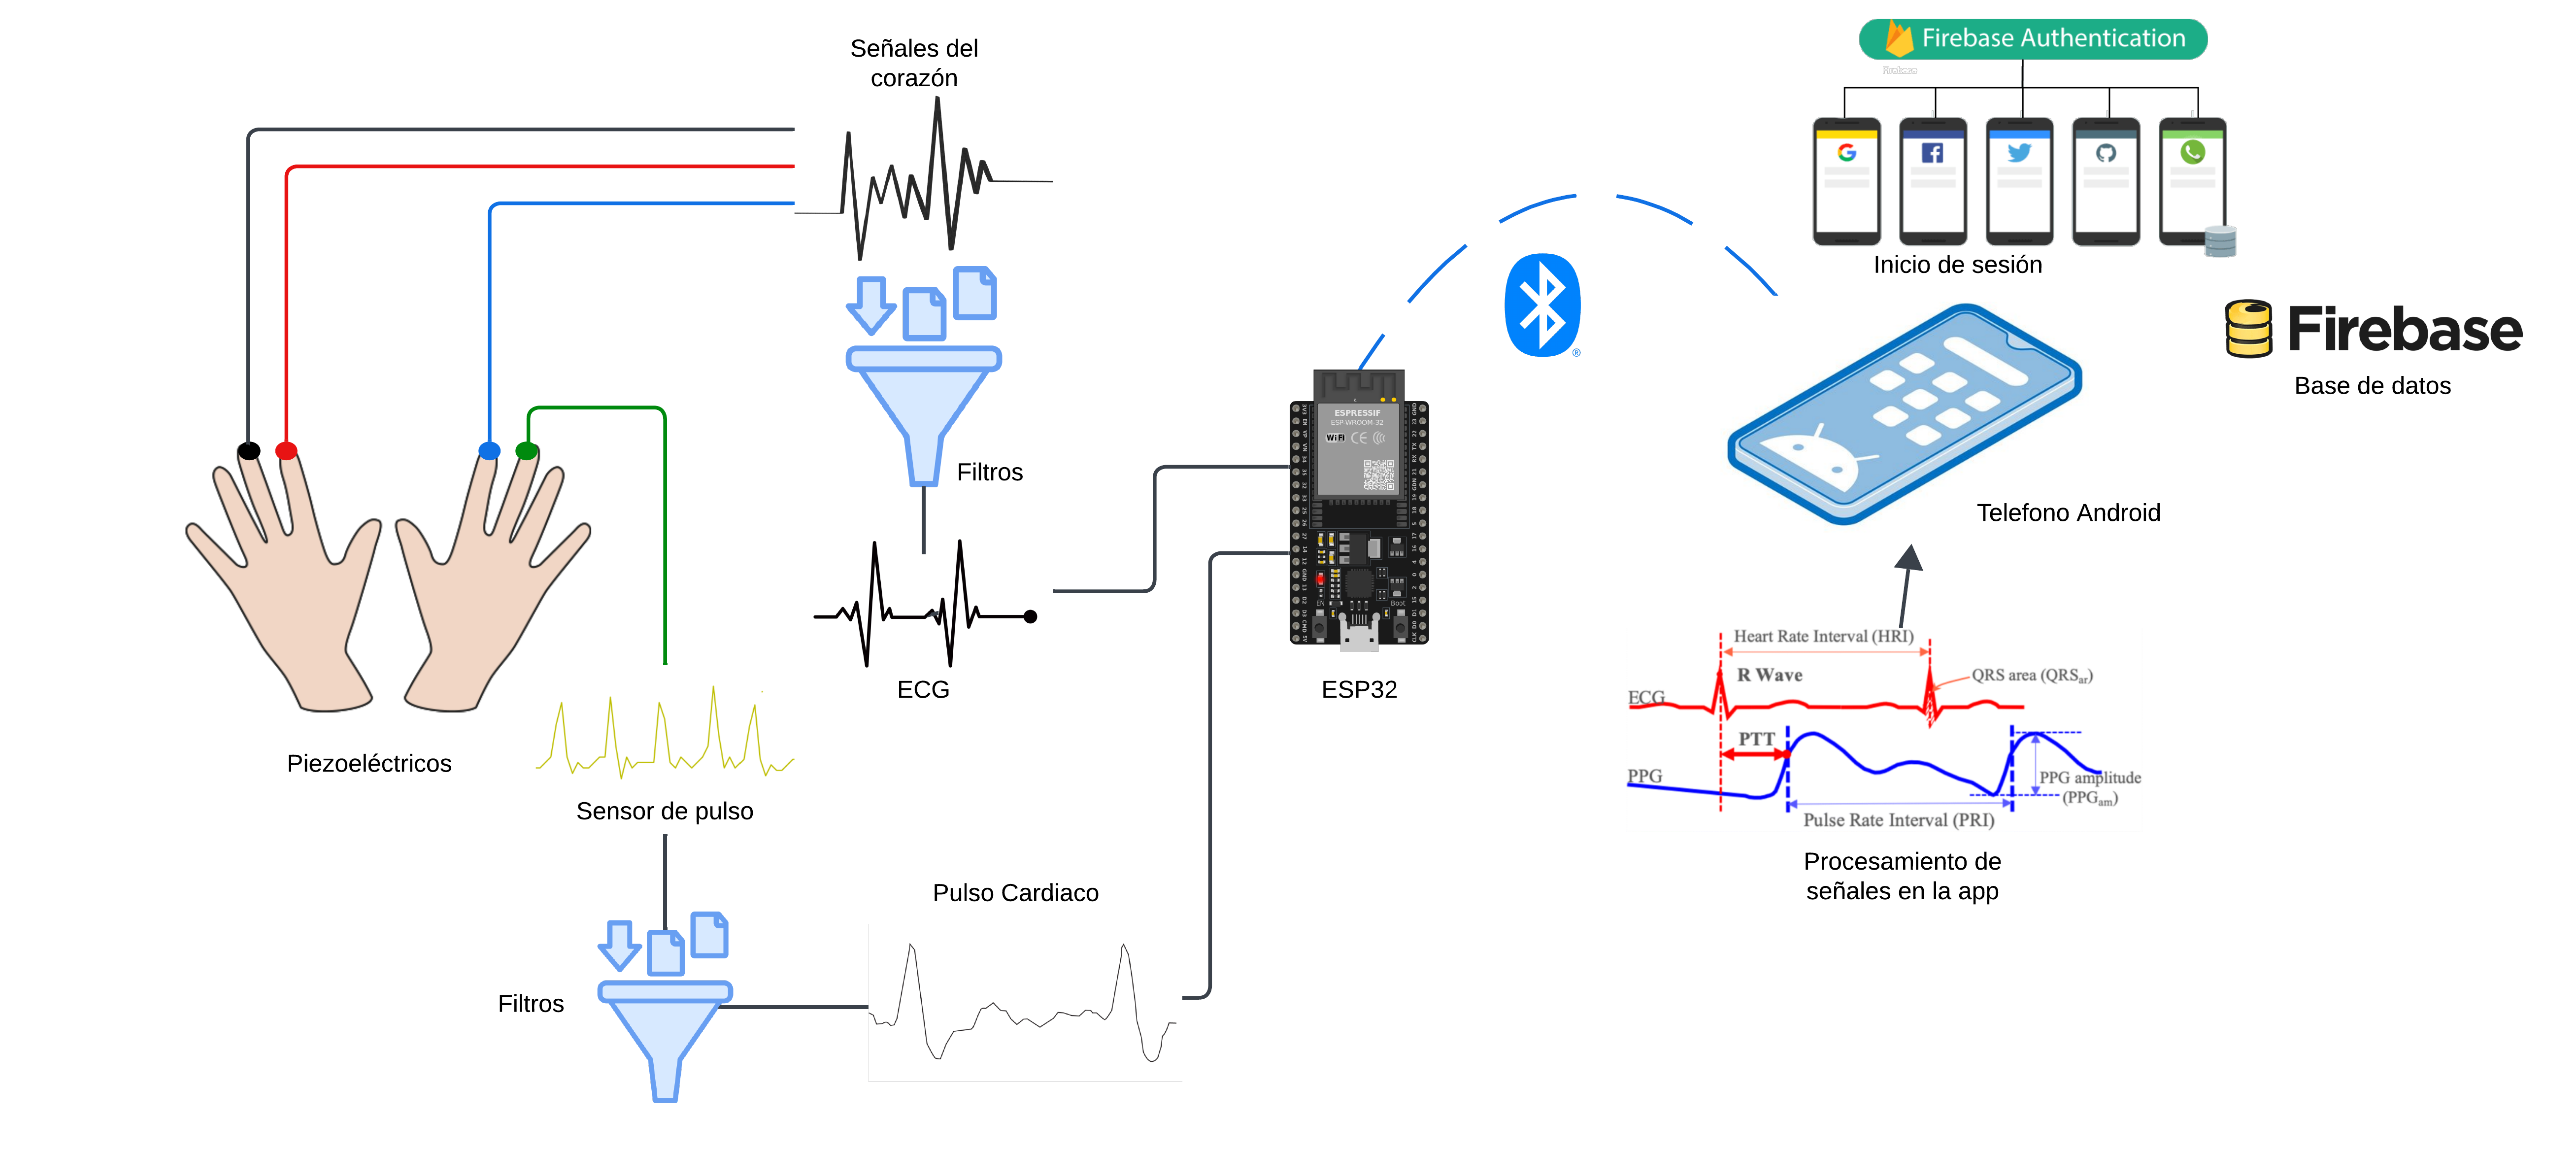
\includegraphics[width=1\textwidth]{img/Desarrollo/flujo_operacion.png}
        \caption[Flujo de operación del sistema.]{Flujo de operación del sistema}
        \label{fig:Flujo_Operacion}
    \end{figure}

    En los siguientes apartados se describen las etapas del flujo de operación del sistema y el desarrollo de cada una de ellas.

    \begin{enumerate}
        \item \textbf{Captura de señales fisiológicas:}
            \begin{itemize}
                \item \textbf{Usuario:} El usuario se coloca los electrodos del ECG y el sensor PPG en los dedos correspondientes para capturar las señales fisiológicas.
                \item \textbf{Electrodos y sensor PPG:} Los electrodos del ECG y el sensor PPG capturan las señales eléctricas y ópticas del cuerpo del usuario.
            \end{itemize}
        \item \textbf{Filtrado y Acondicionamiento de señales:}
            \begin{itemize}
                \item \textbf{ECG}
                    \begin{itemize}
                        \item La señal captada por los electrodos pasa por un amplificador de instrumentación AD620 para aumentar su amplitud.
                        \item Posteriormente, la señal pasa a través de un filtro activo pasa altas y pasa bajas de segundo orden tipo Sallen-Key, el cual elimina el ruido y las frecuencias no deseadas.
                        \item A continuación, se aplica un filtro pasabanda rechazante pasivo RC Twin-T para suprimir el ruido de 60 Hz.
                        \item Finalmente, la señal se amplifica nuevamente mediante un amplificador no inversor, obteniendo así una señal de salida adecuada.
                    \end{itemize}
            \end{itemize}
        \item \textbf{Conversión y Procesamiento Inicial}
            \begin{itemize}
                \item \textbf{ESP32}
                    \begin{itemize}
                        \item La señal del ECG se convierte de analógica a digital mediante un conversor analógico-digital (ADC) de 12 bits.
                        \item La señal del PPG se procesa para eliminar el ruido y las interferencias, y posteriormente se convierte de analógica a digital mediante un ADC de 12 bits.
                    \end{itemize}
            \end{itemize}
        \item \textbf{Transmisión de Datos}
            \begin{itemize}
                \item \textbf{Conectividad Bluetooth}
                    \begin{itemize}
                        \item Se realiza el emparejamiento entre el ESP32 y el teléfono móvil a través de Bluetooth.
                        \item Se envian los datos fisiológicos capturados al teléfono móvil.
                    \end{itemize}
            \end{itemize}
        \item \textbf{Visualización y Análisis en la Aplicación Android}
            \begin{itemize}
                \item \textbf{Recepción de Datos}
                    \begin{itemize}
                        \item La aplicación recibe los datos fisiológicos del ESP32 a través de Bluetooth.
                    \end{itemize}
                \item \textbf{Visualización de los Datos}
                    \begin{itemize}
                        \item Los datos del ECG y PPG se representan de forma gráfica en la interfaz de usuario, ofreciendo una visualización clara del electrocardiograma y del fotopletismograma.
                    \end{itemize}
                \item \textbf{Estimación de la Presión Arterial}
                    \begin{itemize}
                        \item La aplicación realiza un preprocesamiento para calcular el \textit{Pulse Transit Time (PTT)} utilizando la señal del ECG y del PPG.
                        \item A partir del \textit{PTT}, la aplicación estima la presión arterial sistólica y diastólica del usuario.
                    \end{itemize}
            \end{itemize}
    \end{enumerate}

    En la figura~\ref{fig:Diagrama_Secuencia} se muestra el diagrama de secuencia del sistema, que ilustra la interacción entre los componentes del sistema durante la captura, procesamiento y transmisión de datos fisiológicos.

    \begin{figure}[H]
        \centering
        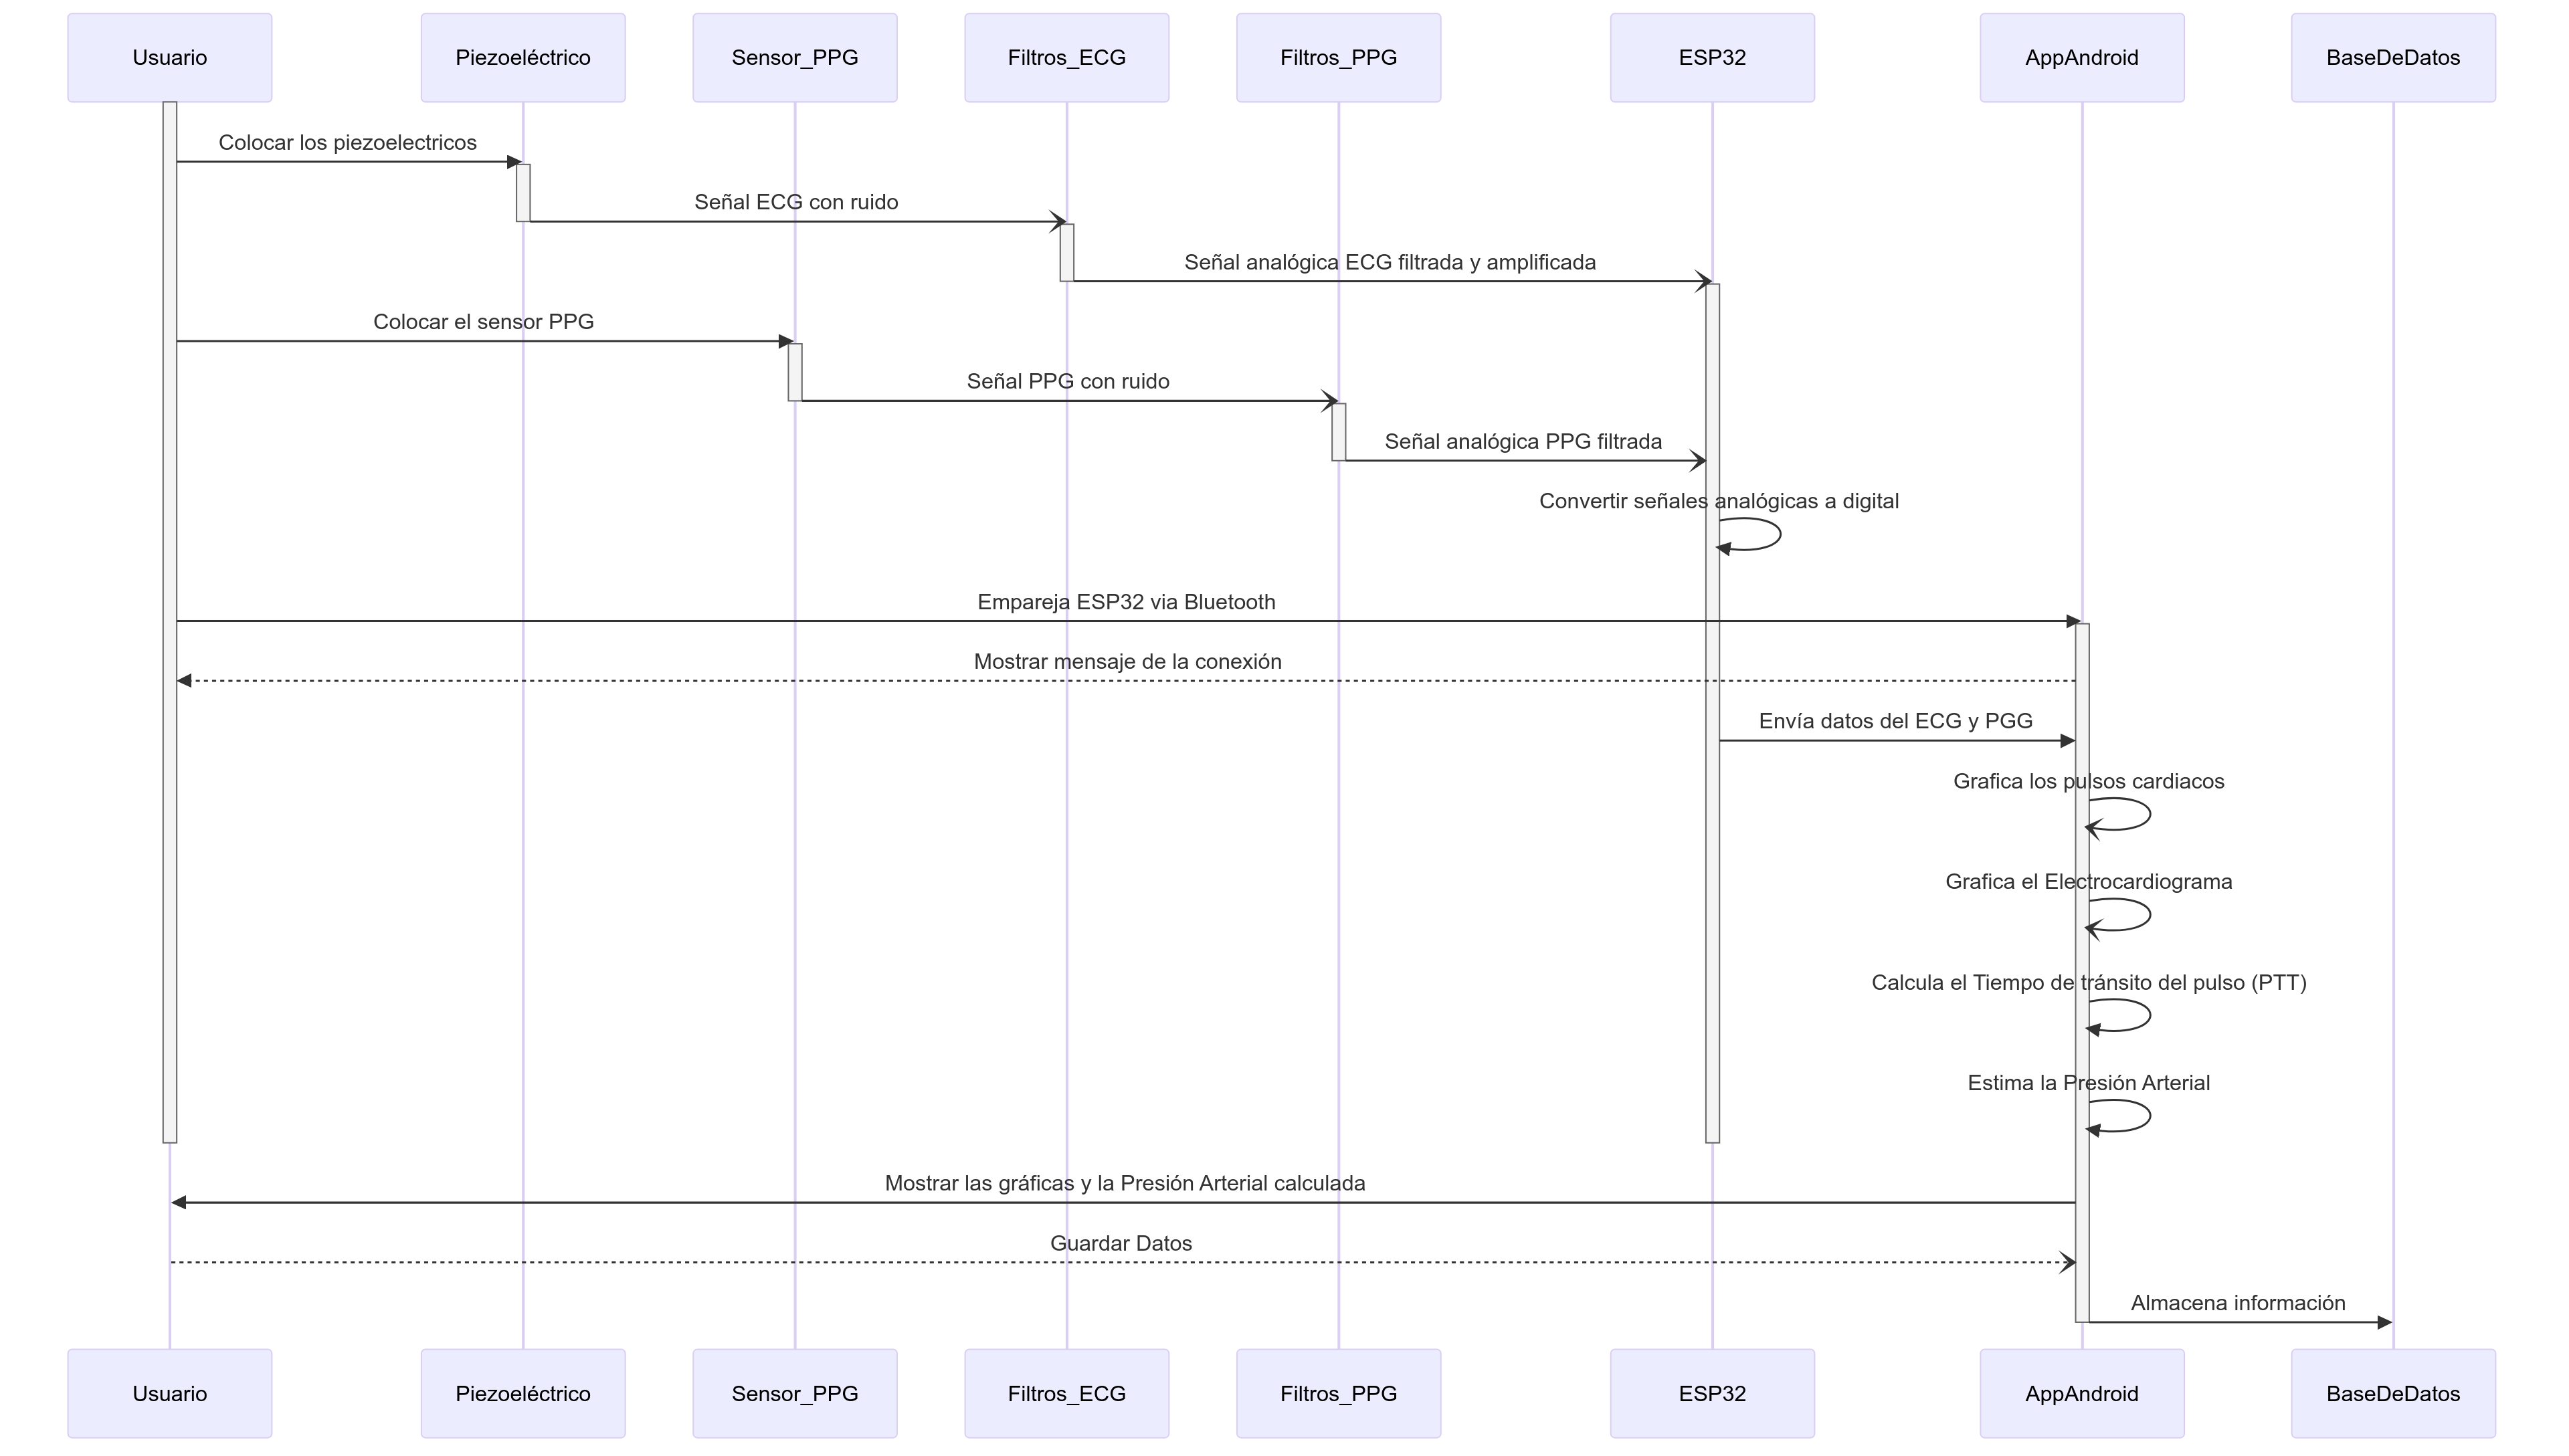
\includegraphics[width=1\textwidth]{img/Desarrollo/diagrama_secuencia.png}
        \caption{Diagrama de secuencia del sistema}
        \label{fig:Diagrama_Secuencia}
    \end{figure}

    \subsection{Desarrollo del circuito de ECG}
        \subsubsection{Amplificador de Instrumentación AD620}
            Para el desarrollo del sistema, comenzamos con el diseño del circuito de ECG utilizando un amplificador de instrumentación AD620, encargado de amplificar la señal captada por los electrodos del ECG. Mediante métodos de prueba y error, se determinó que una ganancia de 21 era necesaria para obtener una señal de salida adecuada.

            Con la ganancia deseada establecida, procedimos a calcular el valor de la resistencia $R_G$, la cual se conecta entre los pines 1 y 8 del AD620. Para ello, partimos de la ecuación~\ref{eq:ganancia_AD620}, que describe la relación entre la ganancia y la resistencia, y la despejamos para obtener la ecuación~\ref{eq:resistencia}, que nos permitió calcular el valor óptimo de $R_G$.

            \begin{equation}
                \label{eq:resistencia}
                R_G = \frac{49.4 k\Omega}{G - 1} = \frac{49.4 k\Omega}{21 - 1} = 2470 \Omega \approx 2.5 k\Omega
            \end{equation}

            Con la resistencia calculada, se procedió a simular el circuito en el software de diseño de circuitos Multisim, obteniendo una ganancia de 20.76, muy cercana a la deseada. La figura~\ref{fig:Simulacion_AD620} muestra la simulación del amplificador de instrumentación AD620 en Multisim.

            \begin{figure}[H]
                \centering
                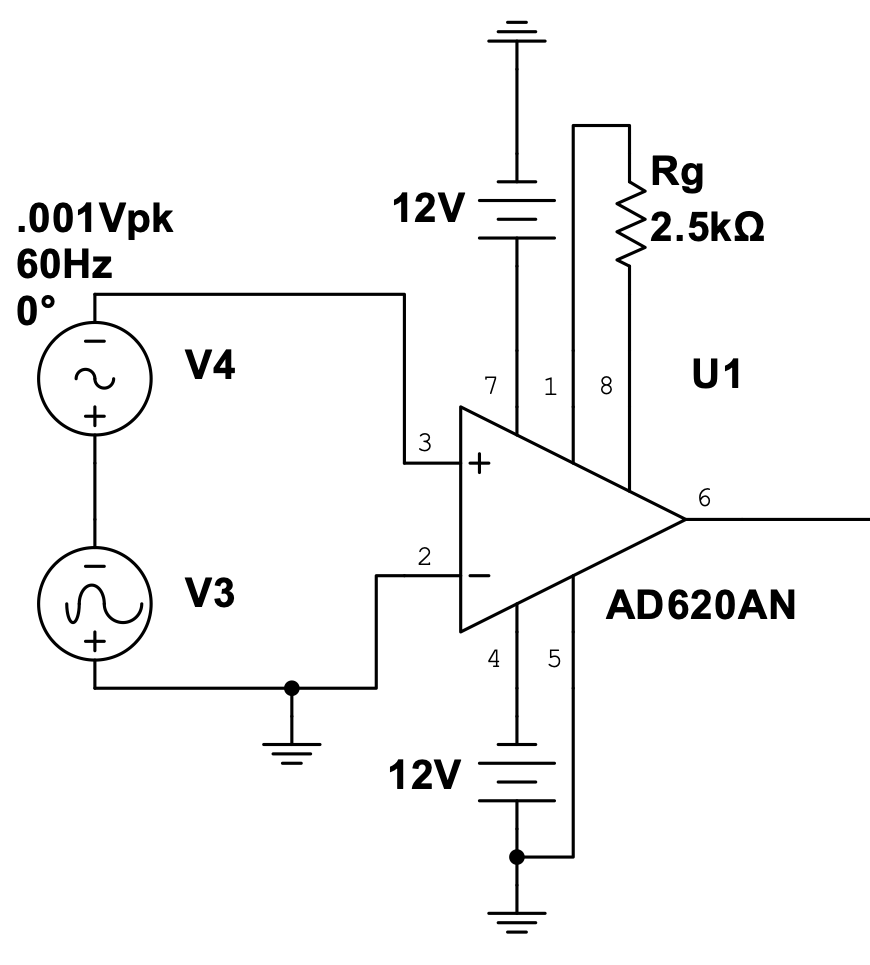
\includegraphics[width=0.5\textwidth]{img/Desarrollo/multisim_AD620AN.png}
                \caption[Simulación del amplificador de instrumentación AD620.]{Simulación del amplificador de instrumentación AD620\footnotemark}
                \label{fig:Simulacion_AD620}
            \end{figure}
            \footnotetext{Muestra la simulación del amplificador de instrumentación AD620 en el software Multisim, con una ganancia de 20.76.}

        \subsubsection{Filtro Activo Pasa Altas}
            Para eliminar el ruido de baja frecuencia presente en la señal de ECG, se implementó un filtro pasa altas de segundo orden tipo \textit{Sallen-Key}. Este filtro permite el paso de frecuencias superiores a una frecuencia de corte, mientras atenúa las frecuencias inferiores a esta.

            En el diseño de este filtro, se utilizó una aproximación de Butterworth debido a su respuesta de frecuencia más plana en la banda de paso, lo que implica la ausencia de sobrepicos en dicha banda y una caída más gradual en la banda de rechazo. Esto contrasta con la aproximación de Chebyshev, que presenta sobrepicos en la banda de paso y una caída más abrupta en la banda de rechazo, o con la aproximación de Bessel,que  ofrece una fase lineal. Los valores de $Q$ y $K$ se obtuvieron de la Tabla~\ref{tab:valores_filtro_pasa_altas}, que presenta los parámetros correspondientes a dicha aproximación.

            \paragraph{Ganancia del Amplificador Operacional}
            Dado que la señal ya fue amplificada en la etapa anterior, se decidió establecer una ganancia unitaria. Por lo tanto, se estableció $R_a$ como infinito (circuito abierto) y $R_b$ como cero (corto circuito), resultando en la Ecuación~\ref{eq:funcion_amplificador_operacional_pasa_altos} para la ganancia del amplificador operacional.

            \begin{equation}
                \label{eq:funcion_amplificador_operacional_pasa_altos}
                A = 1 + \frac{R_b}{R_a} = 1
            \end{equation}

            \paragraph{Cálculo de factor m}
            El factor $m$ es crucial para determinar las resistencias del filtro pasa altos. Se calcula mediante la Ecuación~\ref{eq:factor_m_pasa_altos}.

            \begin{equation}
                \label{eq:factor_m_pasa_altos}
                m = \frac{1+\sqrt{1+8Q^2(A-1)}}{4Q}
            \end{equation}

            Donde:
            \begin{itemize}
                \item $A$: Ganancia del amplificador operacional.
                \item $Q$: Factor de calidad del filtro.
            \end{itemize}

            Para un filtro Butterworth de segundo orden, que ofrece una respuesta en frecuencia plana en la banda de paso, el factor de calidad $Q$ es igual 0.7071. Sustituyendo los valores de $A = 1$ de la Ecuación~\ref{eq:funcion_amplificador_operacional_pasa_altos} y $Q = 0.7071$ en la Ecuación~\ref{eq:factor_m_pasa_altos}, se obtiene el valor de $m$.

            \begin{equation}
                \label{eq:factor_m_pasa_altos_valor}
                m = \frac{1+\sqrt{1+8(0.7071)^2(1-1)}}{4(0.7071)} = \frac{1 + \sqrt{1}}{2.8284}\approx 0.7071
            \end{equation}

            \paragraph{Frecuencia de corte}
            La frecuencia de corte $f_c$ el cual es el punto en el que la señal de salida se atenúa en $-3 dB$, se calcula mediante la Ecuación~\ref{eq:frecuencia_corte_pasa_altos}.
            \begin{equation}
                \label{eq:frecuencia_corte_pasa_altos}
                f_c = \frac{m}{2\pi \cdot k \cdot R_1 \cdot C}
            \end{equation}

            Donde:

            \begin{itemize}
                \item $k$: Constante de la aproximación del filtro.
                \item $R_1$: Resistencia seleccionada.
                \item $C$: Capacitor seleccionada.
            \end{itemize}

            Seleccionamos un valor de $R_1 = 2.2 k\Omega$ y $C = 3.3 \mu F$. Además de que la constante $k$ para una aproximación de Butterworth es 1. Sustituyendo estos valores en la Ecuación~\ref{eq:frecuencia_corte_pasa_altos}, se obtiene la frecuencia de corte del filtro pasa altos.

            \begin{equation}
                \label{eq:frecuencia_corte_pasa_altos_valor}
                f_c = \frac{0.7071}{2\pi \cdot 1 \cdot 2.2 k\Omega \cdot 3.3 \mu F} \approx 15.5 Hz
            \end{equation}

            Esta frecuencia de corte es adecuada para eliminar el ruido de baja frecuencia presente en la señal de ECG.

            \paragraph{Selección de resistencias $R_2$}
            La resistencia $R_2$ se calcula mediante la ecuación~\ref{eq:resistencia_R2_pasa_altos}.

            \begin{equation}
                \label{eq:resistencia_R2_pasa_altos}
                R_2 = \frac{R_1}{m^2} = \frac{2.2 k\Omega}{(0.7071)^2} \approx 4.4 k\Omega 
            \end{equation}

            Se llevó a cabo la simulación del filtro paso alto de segundo orden tipo \textit{Sallen-Key} en Multisim. La Figura~\ref{fig:Simulacion_Filtro_Pasa_Altas} presenta la simulación del filtro en Multisim, utilizando las resistencias y el capacitor seleccionados.

            \begin{figure}[H]
                \centering
                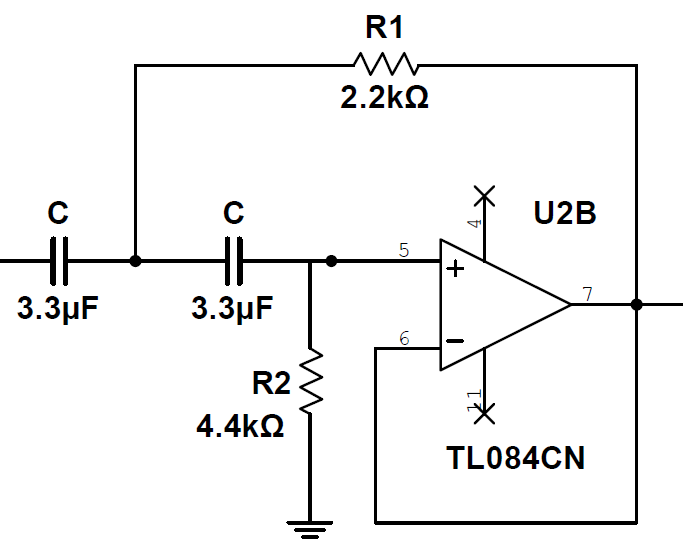
\includegraphics[width=0.6\textwidth]{img/Desarrollo/multisim_pasaAltos.png}
                \caption[Simulación del filtro pasa altas de segundo orden \textit{Sallen-Key}.]{Simulación del filtro pasa altas de segundo orden \textit{Sallen-Key}\footnotemark}
                \label{fig:Simulacion_Filtro_Pasa_Altas}
            \end{figure}
            \footnotetext{Muestra la simulación del filtro pasa altas de segundo orden \textit{Sallen-Key} en el software Multisim, con una frecuencia de corte de 15.5 Hz.}

        \subsubsection{Filtro Activo Pasa Bajos.}

            Para eliminar el ruido de alta frecuencia presente en la señal de ECG, se implementó un filtro pasa bajas de segundo orden tipo \textit{Sallen-Key}. Este filtro permite el paso de frecuencias inferiores a una frecuencia de corte, mientras atenúa las frecuencias superiores a esta.

            En el diseño de este filtro, se utilizó una aproximación de Butterworth y los valores de $Q$ y $K$ se obtuvieron de la Tabla~\ref{tab:valores_filtro_pasa_bajas}, que presenta los parámetros correspondientes a dicha aproximación.

            \paragraph{Ganancia del Amplificador Operacional}
            En este diseño, al igual que con el filtro pasa altas, se busca mantener una ganancia unitaria para evitar amplificar la señal y minimizar la introducción de ruido. Por lo tanto, se establece $R_a = \infty$ (circuito abierto) y $R_b = 0$ (corto circuito), simplificando la ganancia del amplificador operacional a la ecuación~\ref{eq:funcion_amplificador_operacional_pasa_bajos}.

            \begin{equation}
                \label{eq:funcion_amplificador_operacional_pasa_bajos}
                A = 1 + \frac{R_b}{R_a} = 1
            \end{equation}

            \paragraph{Cálculo de factor m}
            El factor $m$ es crucial para determinar las capacitancias del filtro pasa bajas. Se calcula mediante la ecuación~\ref{eq:factor_m_pasa_bajos}.

            \begin{equation}
                \label{eq:factor_m_pasa_bajos}
                m = \frac{1+\sqrt{1+8Q^2(A-1)}}{4Q}
            \end{equation}

            Donde:

            \begin{itemize}
                \item $A$: Ganancia del amplificador operacional.
                \item $Q$: Factor de calidad del filtro.
            \end{itemize}

            Para un filtro Butterworth de segundo orden, que ofrece una respuesta en frecuencia plana en la banda de paso, el factor de calidad $Q$ es igual 0.7071. Sustituyendo los valores de $A = 1$ y $Q = 0.7071$ en la ecuación~\ref{eq:factor_m_pasa_bajos}, se obtiene el valor de $m$.

            \begin{equation}
                \label{eq:factor_m_pasa_bajos_valor}
                m = \frac{1+\sqrt{1+8(0.7071)^2(1-1)}}{4(0.7071)} = \frac{1 + \sqrt{1}}{2.8284}\approx 0.7071
            \end{equation}

            \paragraph{Frecuencia de corte}
            La frecuencia de corte $f_c$ el cual es el punto en el que la señal de salida se atenúa en $-3 dB$, se calcula mediante la ecuación~\ref{eq:frecuencia_corte_pasa_bajos}.

            \begin{equation}
                \label{eq:frecuencia_corte_pasa_bajos}
                f_c = \frac{1}{2\pi \cdot k \cdot R \cdot m \cdot C_1}
            \end{equation}

            Donde:
            \begin{itemize}
                \item $k$: Constante de la aproximación del filtro.
                \item $R$: Resistencia seleccionada.
                \item $C_1$: Capacitancia seleccionada.
            \end{itemize}

            Seleccionamos un valor de $R = 2.7 k\Omega$ y $C_1 = 4.7 \mu F$. Además de que la constante $k$ para una aproximación de Butterworth es 1. Sustituyendo estos valores en la ecuación~\ref{eq:frecuencia_corte_pasa_bajos}, se obtiene la frecuencia de corte del filtro pasa bajos.

            \begin{equation}
                \label{eq:frecuencia_corte_pasa_bajos_valor}
                f_c = \frac{1}{2\pi \cdot 1 \cdot 2.7 k\Omega \cdot 0.7071\cdot 4.7 \mu F} = \frac{1}{2\pi \cdot 2.7 x10^3 \cdot 0.7071\cdot 4.7 x10^{-6}} \approx 17.737 Hz
            \end{equation}

            Esta frecuencia de corte es adecuada para eliminar el ruido de alta frecuencia presente en la señal de ECG.

            \paragraph{Cálculo de la capacitancia C2}
            La capacitancia $C_2$ se calcula mediante la ecuación~\ref{eq:capacitancia_C2_pasa_bajos}.

            \begin{equation}
                \label{eq:capacitancia_C2_pasa_bajos}
                C_2 = m^2 \cdot C_1 = (0.7071)^2 \cdot 4.7 \mu F \approx 2.35 \mu F
            \end{equation}

            Se seleccionó un valor de $C_2 = 2.2 \mu F$, ya que es el valor comercial más cercano al calculado.

            \begin{equation}
                C_2 = 2.2 \mu F
            \end{equation}

            Se llevó a cabo la simulación del filtro pasa bajas de segundo orden tipo \textit{Sallen-Key} en Multisim. 
            %La Figura~\ref{fig:Simulacion_Filtro_Pasa_Bajas} presenta la simulación del filtro en Multisim, utilizando las resistencias y los capacitores seleccionados.
            
        \subsubsection{Filtro Notch Pasivo Rechaza Banda RC Twin-T}
                En la etapa de acondicionamiento de la señal, se implementó un filtro notch pasivo RC tipo Twin-T para atenuar las interferencias de 60 Hz, comúnmente presentes debido al ruido de la red eléctrica. Este filtro es eficaz para eliminar una frecuencia específica sin afectar significativamente las demás componentes de la señal.

                El filtro Twin-T es un circuito pasivo que utiliza resistencias y capacitores dispuestos en una configuración en forma de "T" doble, lo que permite rechazar una frecuencia central $f_0$. Al ser un filtro pasivo, está compuesto únicamente por resistencias y capacitores, lo que simplifica su diseño y construcción. Sin embargo, su factor de calidad $Q$ es limitado, generalmente por debajo de 0.5, lo que implica un ancho de banda relativamente amplio en comparación con filtros activos. En otras palabras, si tenemos una frecuencia central de 100 Hz, el ancho de banda del filtro será de 200 Hz.

                Para diseñar el filtro notch pasivo RC Twin-T centrado en $f_0 = 60 Hz$, se utilizaron las siguientes ecuaciones:

                Seleccionamos los parámetros iniciales del filtro:
                \begin{itemize}
                    \item Frecuencia central $(f_0) = 60 Hz$
                    \item Factor de calidad $(Q) = 0.25$
                    \item Capacitancia base $(C_1) = 100 nF$
                \end{itemize}

                \subparagraph{Cálculo de la resistencia R1}
                    La resistencia $R_1$ se calcula mediante la ecuación~\ref{eq:resistencia_R1_notch}.

                    \begin{equation}
                        \label{eq:resistencia_R1_notch}
                        R_1 = \frac{1}{4\pi \cdot f_0 \cdot Q \cdot C_1}
                    \end{equation}

                    Sustituyendo los valores de $f_0 = 60 Hz$, $Q = 0.25$ y $C_1 = 100 nF$ en la ecuación~\ref{eq:resistencia_R1_notch}, se obtiene el valor de $R_1$.

                    \begin{equation}
                        R_1 = \frac{1}{4\pi \cdot 60 Hz \cdot 0.25 \cdot 100 nF} = 53051.6477 \Omega \approx 53 k\Omega
                    \end{equation}

                \subparagraph{Cálculo de la resistencia R2}
                    La resistencia $R_2$ se calcula mediante la ecuación~\ref{eq:resistencia_R2_notch}.

                    \begin{equation}
                        \label{eq:resistencia_R2_notch}
                        R_2 = \frac{1}{2\pi \cdot f_0 \cdot C_1}
                    \end{equation}

                    Sustituyendo los valores en la ecuación~\ref{eq:resistencia_R2_notch}, se obtiene el valor de $R_2$.

                    \begin{equation}
                        R_2 = \frac{1}{2\pi \cdot 60 Hz \cdot 100 nF} = 26.5258 k\Omega \approx 26 k\Omega
                    \end{equation}

                \subparagraph{Cálculo de la capacitancia C2}
                    La capacitancia $C_2$ se calcula mediante la ecuación~\ref{eq:capacitancia_C2_notch}.

                    \begin{equation}
                        \label{eq:capacitancia_C2_notch}
                        C_2 = 2Q \cdot C_1
                    \end{equation}

                    Sustituyendo el valor de $C_1 = 100 nF$ en la ecuación~\ref{eq:capacitancia_C2_notch}, se obtiene el valor de $C_2$.

                    \begin{equation}
                        C_2 = 2(0.25) \cdot 100 nF = 50 nF
                    \end{equation}

                \subparagraph{Cálculo de la capacitancia C3}
                    La capacitancia $C_3$ se calcula mediante la ecuación~\ref{eq:capacitancia_C3_notch}.

                    \begin{equation}
                        \label{eq:capacitancia_C3_notch}
                        C_3 = (1 - 2Q) \cdot C_1
                    \end{equation}

                    Sustituyendo los valores, tenemos que:

                    \begin{equation}
                        C_3 = (1 - 2(0.25)) \cdot 100 nF = 50 nF
                    \end{equation}

            \paragraph{Amplificador no Inversor}
                Finalmente, para visualizar la señal, es necesario amplificar nuevamente la señal ya acondicionada antes de su observación en el osciloscopio. Para ello, un amplificador no inversor sencillo es adecuado para cumplir con esta tarea. A continuación se muestra la ecuación~\ref{eq:ganancia_amplificador_no_inversor} para calcular la ganancia del amplificador no inversor.

                \begin{equation}
                    \label{eq:ganancia_amplificador_no_inversor}
                    A = 1 + \frac{R_F}{R_{1}} = 1 + \frac{1 M\Omega}{10 k\Omega} = 101
                \end{equation}

                Donde $R_f$ es la resistencia de realimentación y $R_g$ es la resistencia de ganancia. Este diseño asegura que la señal amplificada mantenga la fidelidad necesaria para una visualización precisa en el osciloscopio.


